%%%%%%%%%%%%%%%%%%%%%%%%%%%%%%%%%%%%%%%%%%%%%%%%%%%%%%%%%%%%%%%%%%%%%%%%%%%%%%%%
%2345678901234567890123456789012345678901234567890123456789012345678901234567890
%        1         2         3         4         5         6         7         8

\documentclass[letterpaper, 10 pt, conference]{ieeeconf}  % Comment this line out if you need a4paper

% \documentclass[a4paper, 10pt, conference]{ieeeconf}      % Use this line for a4 paper

\IEEEoverridecommandlockouts                              % This command is only needed if 

\overrideIEEEmargins                                      % Needed to meet printer requirements.

\usepackage{amsmath,amssymb,amsfonts}
\usepackage{tikz}                                                          % you want to use the \thanks command
\usepackage[T1]{fontenc}
\usepackage[utf8]{inputenc}
\usepackage{xcolor,colortbl}
\usepackage{subcaption}
\graphicspath{ {images/} } 
\usepackage{blindtext}
\usepackage{subfiles}
\usepackage{algorithm}
\usepackage{algpseudocode}
\usepackage{multicol}
% \usepackage{float}
\usepackage{stfloats}
\usepackage{array}
%\usepackage[maxfloats=256]{morefloats}
%\maxdeadcycles=15000
\usepackage{url}
\usepackage{diagbox}
\usepackage{flushend}
\usepackage{lipsum}
\usepackage[verbose]{placeins} 
\usepackage{multirow}
\usetikzlibrary{arrows.meta, positioning}
\usepackage{subcaption}
\newtheorem{theorem}{\normalfont\textbf{Theorem}}
\newtheorem{problem}{\normalfont\textbf{Problem}}
\newcommand{\mycomment}[1]{}
\newcommand{\algrule}[1][.2pt]{\par\vskip.5\baselineskip\hrule height #1\par\vskip.5\baselineskip}
\newcolumntype{C}[1]{>{\centering\arraybackslash}p{#1}}
\newcolumntype{M}[1]{>{\centering\arraybackslash}m{#1}}
\let\labelindent\relax  % Redefine before loading enumitem
\usepackage{enumitem}
\newcommand{\purplecircle}{\textcolor{blue}{\textbullet}}
\newcommand{\largepurplecircle}{\textcolor{blue}{\scalebox{1.5}{$\bullet$}}}
\newcommand{\CRD}{$\text{C}_{\text{R}} \text{D }$}
\newcommand{\qedwhite}{\hfill \ensuremath{\Box}}
\newcommand{\mathbbmI}[1]{\mathbb{I}\left(#1\right)}
%\newcommand{\DoTikzmark}[1]{%
%  \tikz[remember picture] \coordinate[shift={(0,.7ex)}](#1);%
%}
%\newcommand{\colrow}[3][]{%
%  \tikz[overlay,remember picture, line width=10pt]
%    \draw[shorten >=-.1em, shorten <=-.1em, #1] (#2)--(#3);
%}

%\newcommand{\mc}[2]{\multicolumn{#1}{c}{#2}}
%\definecolor{Gray}{gray}{0.85}
%\definecolor{LightCyan}{rgb}{0.88,1,1}

%\newcolumntype{a}{>{\columncolor{Gray}}c}
%\newcolumntype{b}{>{\columncolor{white}}c}

%\newenvironment{remark}{
%  \par\medskip
%  \noindent\textbf{\textcolor{blue}{Remark.}} \ignorespaces
%  \color{red}\itshape
%}{
%  \par\medskip
%}







% \title{\LARGE \bf Finding the Balance: Cyclist Safety vs. Car Flow Efficiency}
% \title{\LARGE \bf A Bi-Level Optimization Framework for Budget-Efficient Cycling  \\  Infrastructure Upgrades with Traffic Impact Mitigation}
\title{\LARGE \bf Safety-Oriented Design of Cycling Infrastructure\\Minimizing Impact on Vehicular Traffic}
%Graph-Metric to Asses Safety/Stress in Large-Scale Bike Mobility Networks
% \author{Manuel Campero Jurado, Mauro Salazar, Giovanni De Nunzio, Carlos Canudas-de-Wit}
\author{Manuel Campero Jurado$^{1}$, Giovanni De Nunzio$^{2}$, Carlos Canudas-de-Wit$^{1}$ % <-this % stops a space
 % stops a space
\thanks{$^{1}$Univ. Grenoble Alpes, Inria, CNRS, Grenoble INP, GIPSA-Lab, 38000 Grenoble, France
        {\footnotesize \{\textit{manuel.campero-jurado@inria.fr, carlos.canudas-de-wit@gipsa-lab.fr}\} }}%
\thanks{$^{2}$IFP Energies nouvelles,
Rond-point de l’échangeur de Solaize, BP 3, 69360 Solaize, France,
        {\footnotesize \{\textit{giovanni.de-nunzio@ifpen.fr}\}}}%
%
}



\begin{document}



\maketitle
% \thispagestyle{plain}
% \pagestyle{plain}
\pagestyle{empty}


%%%%%%%%%%%%%%%%%%%%%%%%%%%%%%%%%%%%%%%%%%%%%%%%%%%%%%%%%%%%%%%%%%%%%%%%%%%%%%%%
\begin{abstract}
Designing safer cycling infrastructure without causing major traffic delays is a key challenge in city planning. This paper presents a bi-level optimization framework to address and solve this problem. The upper level plans bike lane upgrades to reduce cyclists' exposure to traffic, while ensuring car travel times remain reasonable despite potential impacts on road capacity. The lower level models and determines cyclists’ route choices based on factors such as slope, turns, and traffic conditions on bike paths. We present a case study for Grenoble network, France, and a safety-oriented upgrade of the existing cycling infrastructure is determined using a genetic algorithm. To understand how cars are affected by such a modification of the cycling infrastructure, we simulate how drivers might change their routes after bike lanes upgrades. Our results show that cyclists' safety can be improved with only small impacts on car travel times, thus highlighting the potential of this approach to support safer, more sustainable urban mobility.
% Promoting safe and efficient cycling infrastructure is a key challenge in urban transportation planning, especially when balancing strategies that improve cyclist safety while moderating the impact on overall traffic performance. This paper presents a bi-level optimization framework for strategic cycling infrastructure planning, where the upper level aims to reduce cyclists' exposure to vehicular traffic while minimizing the impact on car travel times, and the lower-level problem models cyclists' route choice using an all-or-nothing assignment. We apply this framework to the cycling network of Grenoble, France, using a genetic algorithm optimizer. To assess the impact on car traffic, we simulate traffic redistribution after upgrades by solving a user equilibrium traffic assignment reflecting drivers' adjusted route choices. Results show that our trade-off approach achieves significantly lower cyclist exposure with only minor increases in vehicle travel times, validating the effectiveness of our method in improving cycling safety without significant disruption of vehicular flow.
\end{abstract}

\begin{keywords}
Cycling infrastructure, bi-level optimization, safety,  urban planning, traffic assignment.
\end{keywords}




%%%%%%%%%%%%%%%%%%%%%%%%%%%%%%%%%%%%%%%%%%%%%%%%%%%%%%%%%%%%%%%%%%%%%%%%%%%%%%%%
% \section{Introduction} 

% Cycling offers many benefits for health, the environment, and the economy, such as lowering emissions, reducing travel expenses, and supporting public health \cite{garrard2012health, gotschi2016cycling}. Because of this, authorities are increasingly encouraging it as a sustainable option for short-distance travel. However, concerns about safety and comfort continue to be major obstacles to more widespread adoption \cite{fishman2012barriers}. Studies show that physically separated bike lanes significantly improve these perceptions and boost ridership \cite{lawrence2018cyclist}. Well-connected high-quality infrastructure further encourages cycling \cite{pucher2011walking}. However, allocating space for bike lanes often reduces the capacity of adjacent car lanes, potentially increasing congestion and travel times. Therefore, under budget constraints, cities must carefully prioritize investments to improve cyclist safety and comfort without significantly impacting car travel times. This paper proposes a framework to address this challenge.



% \textit{Related Work:}  
% The optimization of the cycling infrastructure has been studied through various lenses. One common approach is to identify network links to upgrade for improving bike connectivity while minimizing car travel time \cite{mesbah2012bilevel, smith2012mathematical}. In \cite{wiedemann2025bike}, a planning framework is introduced that simultaneously improves bike infrastructure and preserves car accessibility, using a multi-criteria optimization to balance bike and car travel times and explore trade-offs in lane reallocation. Other methods, such as in \cite{mahfouz2023road}, prioritize upgrading bike lanes along segments with high potential cycling demand, while ensuring that these improvements do not significantly disrupt car traffic performance. Similarly, \cite{shui2019optimization, folco2023data} propose optimization models under budget constraints using heuristic methods to design efficient bike lane networks that affect only selected lanes that do not greatly affect automobile traffic.

% Studies in \cite{paulsen2023societally, duthie2014optimization} focus on maximizing the societal benefit-cost ratio of bicycle infrastructure, improving network connectivity and economic feasibility. However, these approaches often emphasize improvements to the cycling network without explicit consideration of their effects on automobile traffic, or both objectives often seek to reduce travel time for automobiles and bicycles, without considering safety for cyclists. This paper addresses this gap by proposing a new planning framework that explicitly accounts for both safety and traffic dynamics in bicycle infrastructure decisions, which to the best of our knowledge, has not been previously developed.

% \begin{figure}[t]
% \vspace{0.2cm}
%   \centering
%  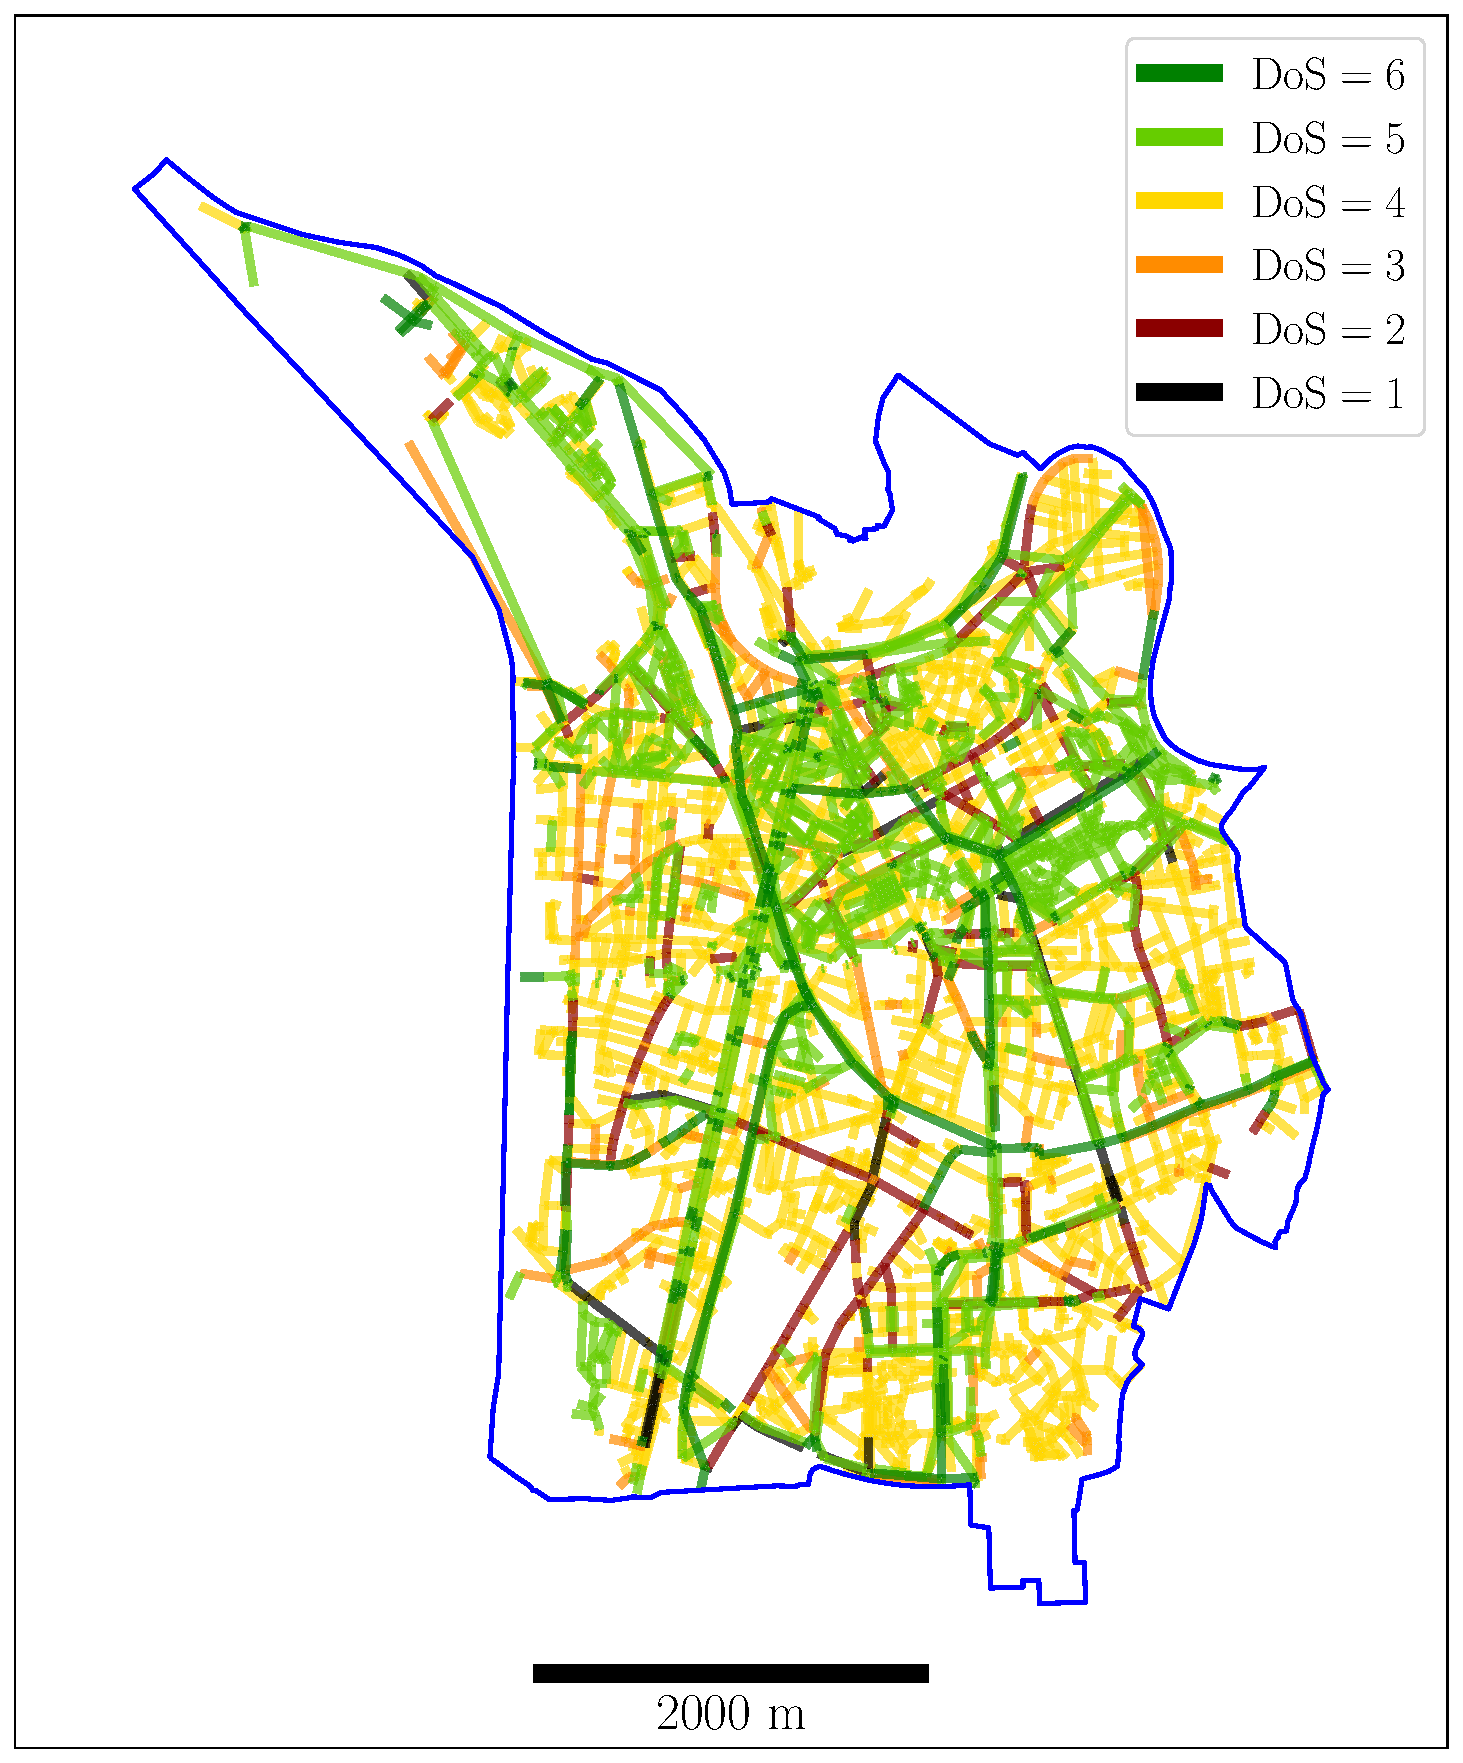
\includegraphics[width=0.48\linewidth]{Images/bikes_network.pdf}
%   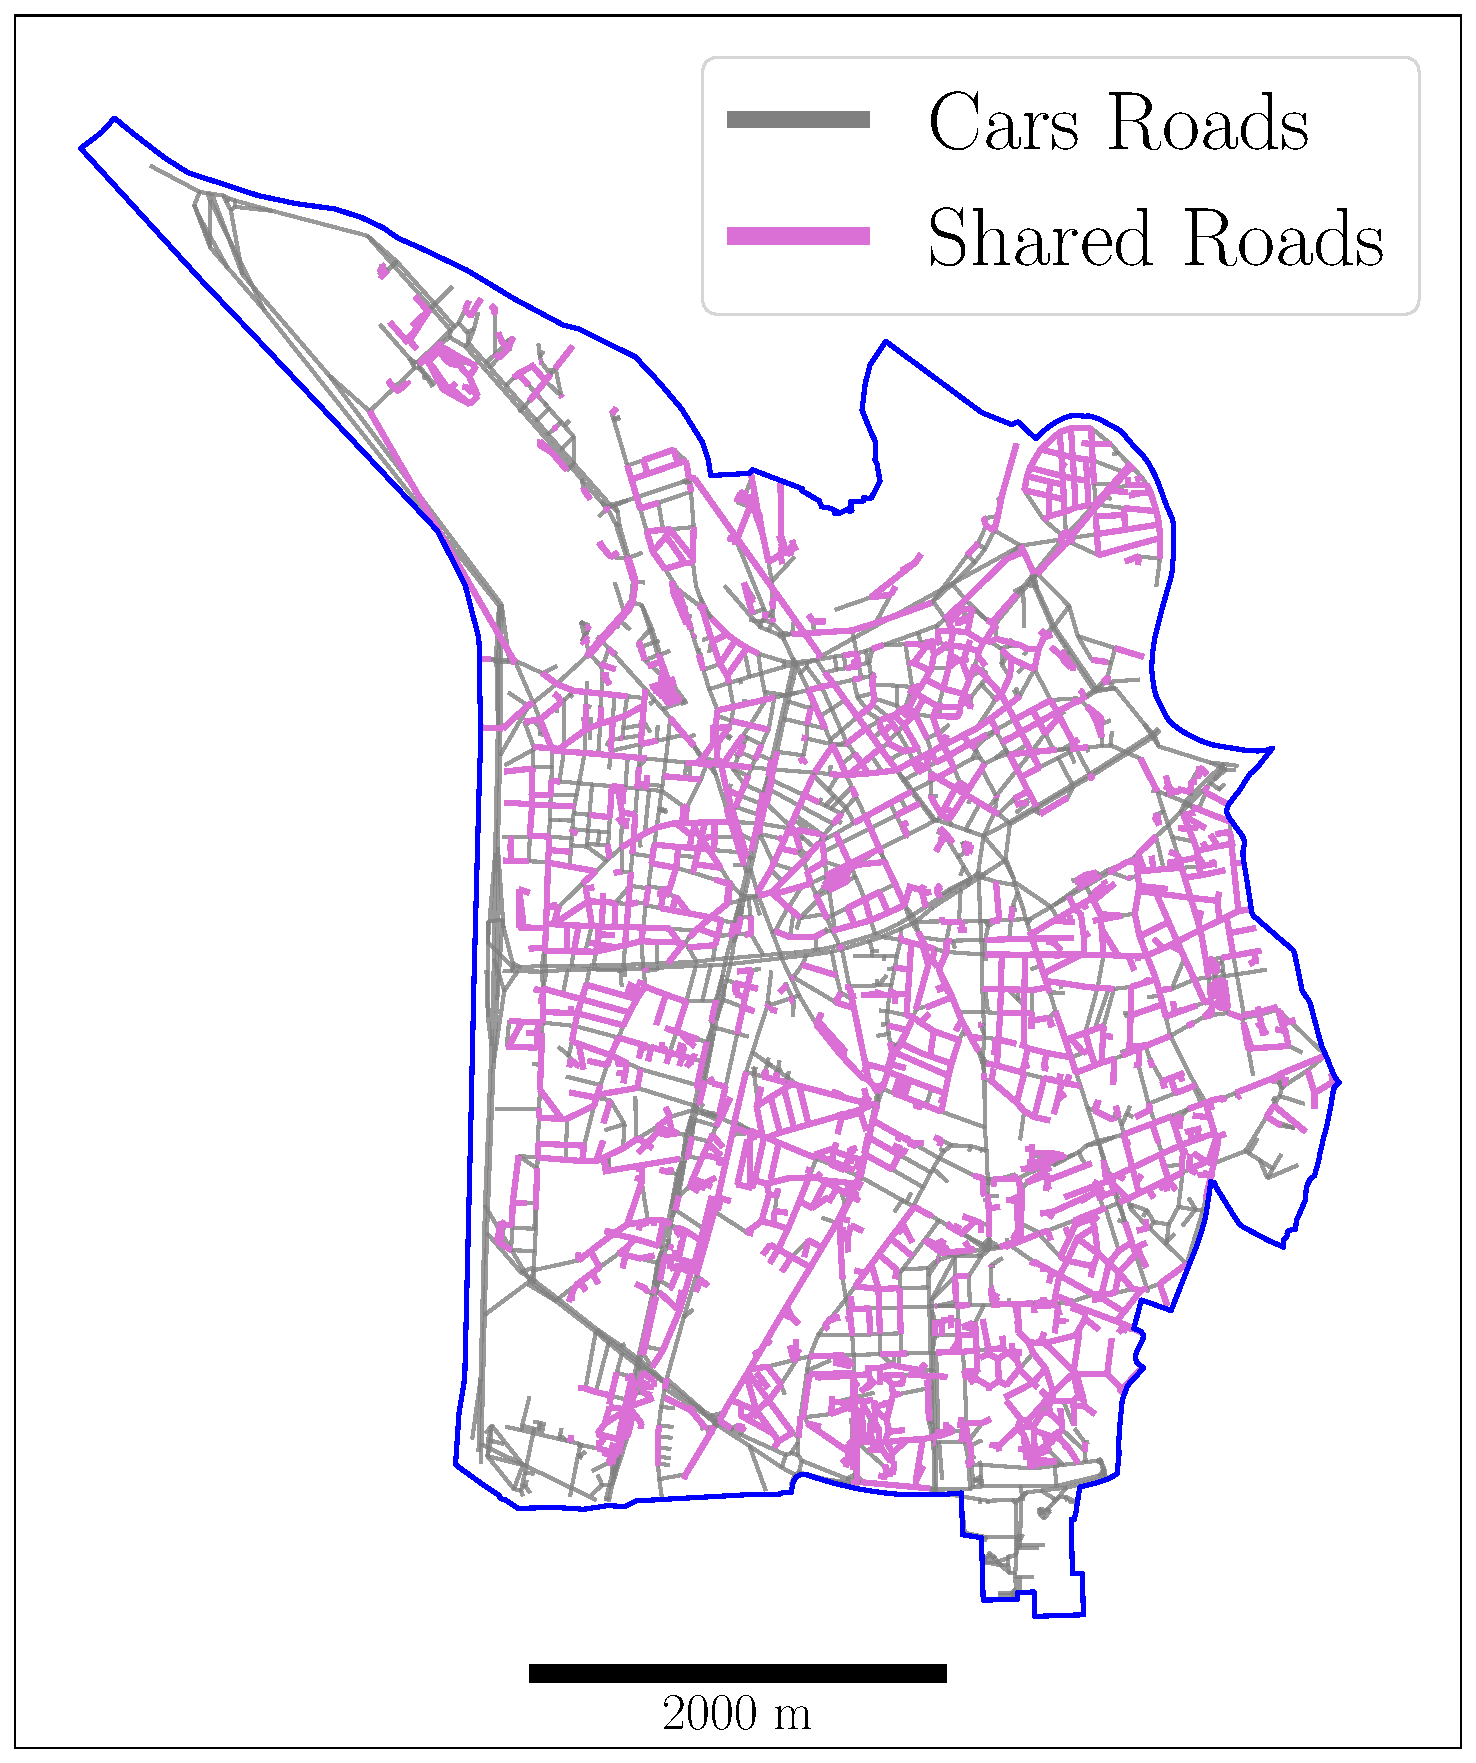
\includegraphics[width=0.48\linewidth]{Images/cars_network.pdf}
%   \caption{\footnotesize Multi-modal transportation network of Grenoble, France. \textit{Left:} Cycling infrastructure classified by degree of separation (DoS) of bike lanes, ranging from 1 (least separated) to 6 (fully separated). \textit{Right:} Road network for cars, including links shared with bicycles.}
%   \label{multi_network}
% \end{figure}



% \textit{Statement of Contributions:} This paper introduces a bi-level optimization framework for upgrading cycling infrastructure based on a six-level classification of bike lanes by degree of separation (DoS) from motor traffic. Higher DoS categories offer greater safety and comfort by reducing exposure to cars. Unlike previous approaches, our method jointly minimizes cyclists' exposure and car travel time impacts, while accounting for induced shifts in cyclist flow due to infrastructure upgrades. Key contributions include: (1) a cyclist flow estimation model that integrates slope, turning angles, and annual average daily traffic (AADT) into route choice modeling; (2) a novel bi-level optimization approach combining cycling infrastructure upgrade planning and car flow traffic assignment, applied to the Grenoble network; and (3) an evaluation strategy comparing fixed-route and post-upgrade user equilibrium traffic assignment to validate the robustness of the planning assumptions. Results demonstrate that substantial improvements in cyclists safety can be achieved with minimal disruption to car travel times.



% \textit{Organization:} The remainder of this paper is structured as follows. Section~\ref{model_design} introduces the data sources, bike lane classification, and overall model design, including the assignment methods for both bike and car flows. Section~\ref{solution_algorithm} presents the algorithm used to solve the bi-level problem. Section~\ref{case_study} details a case study of the Grenoble network. Finally, Section~\ref{conclusions} summarizes the key findings and discusses directions for future research.


\section{Introduction} 

Cycling brings substantial benefits to health, the environment, and the economy by lowering emissions, reducing travel costs, and promoting public health \cite{garrard2012health}. Consequently, it is increasingly promoted as a sustainable mode for short trips. Yet, safety and comfort concerns remain major barriers to broader adoption \cite{fishman2012barriers}. Research shows that physically separated bike lanes improve perceived safety and encourage cycling \cite{lawrence2018cyclist}, and that well-connected infrastructure further promotes usage \cite{pucher2011walking}. However, reallocating road space for bikes may reduce car lane capacity, raising concerns about congestion. Given limited budgets, cities must strategically invest to enhance cyclist safety and comfort while minimizing impacts on car travel. This paper presents a framework to support such decisions.

\textit{Related Work:}  
Cycling infrastructure planning has been approached from multiple angles. Some works focus on selecting links to upgrade to improve bike connectivity while limiting car travel time increases \cite{mesbah2012bilevel, smith2012mathematical}. The framework in \cite{wiedemann2025bike} balances bike and car travel times through multi-criteria optimization. Other approaches, such as \cite{mahfouz2023road}, prioritize high-demand corridors while limiting car traffic disruption. Similarly, \cite{shui2019optimization} uses heuristics to design cost-effective bike networks under budget limits, minimizing car impacts.

Studies like \cite{paulsen2023societally, duthie2014optimization} aim to maximize the societal benefit-cost ratio of cycling infrastructure, focusing on connectivity and feasibility. However, many omit direct safety considerations or model both modes with travel time as the only objective. This paper fills that gap by integrating safety and traffic dynamics into infrastructure planning—a combination not previously addressed.

\begin{figure}[t]
\vspace{0.2cm}
  \centering
 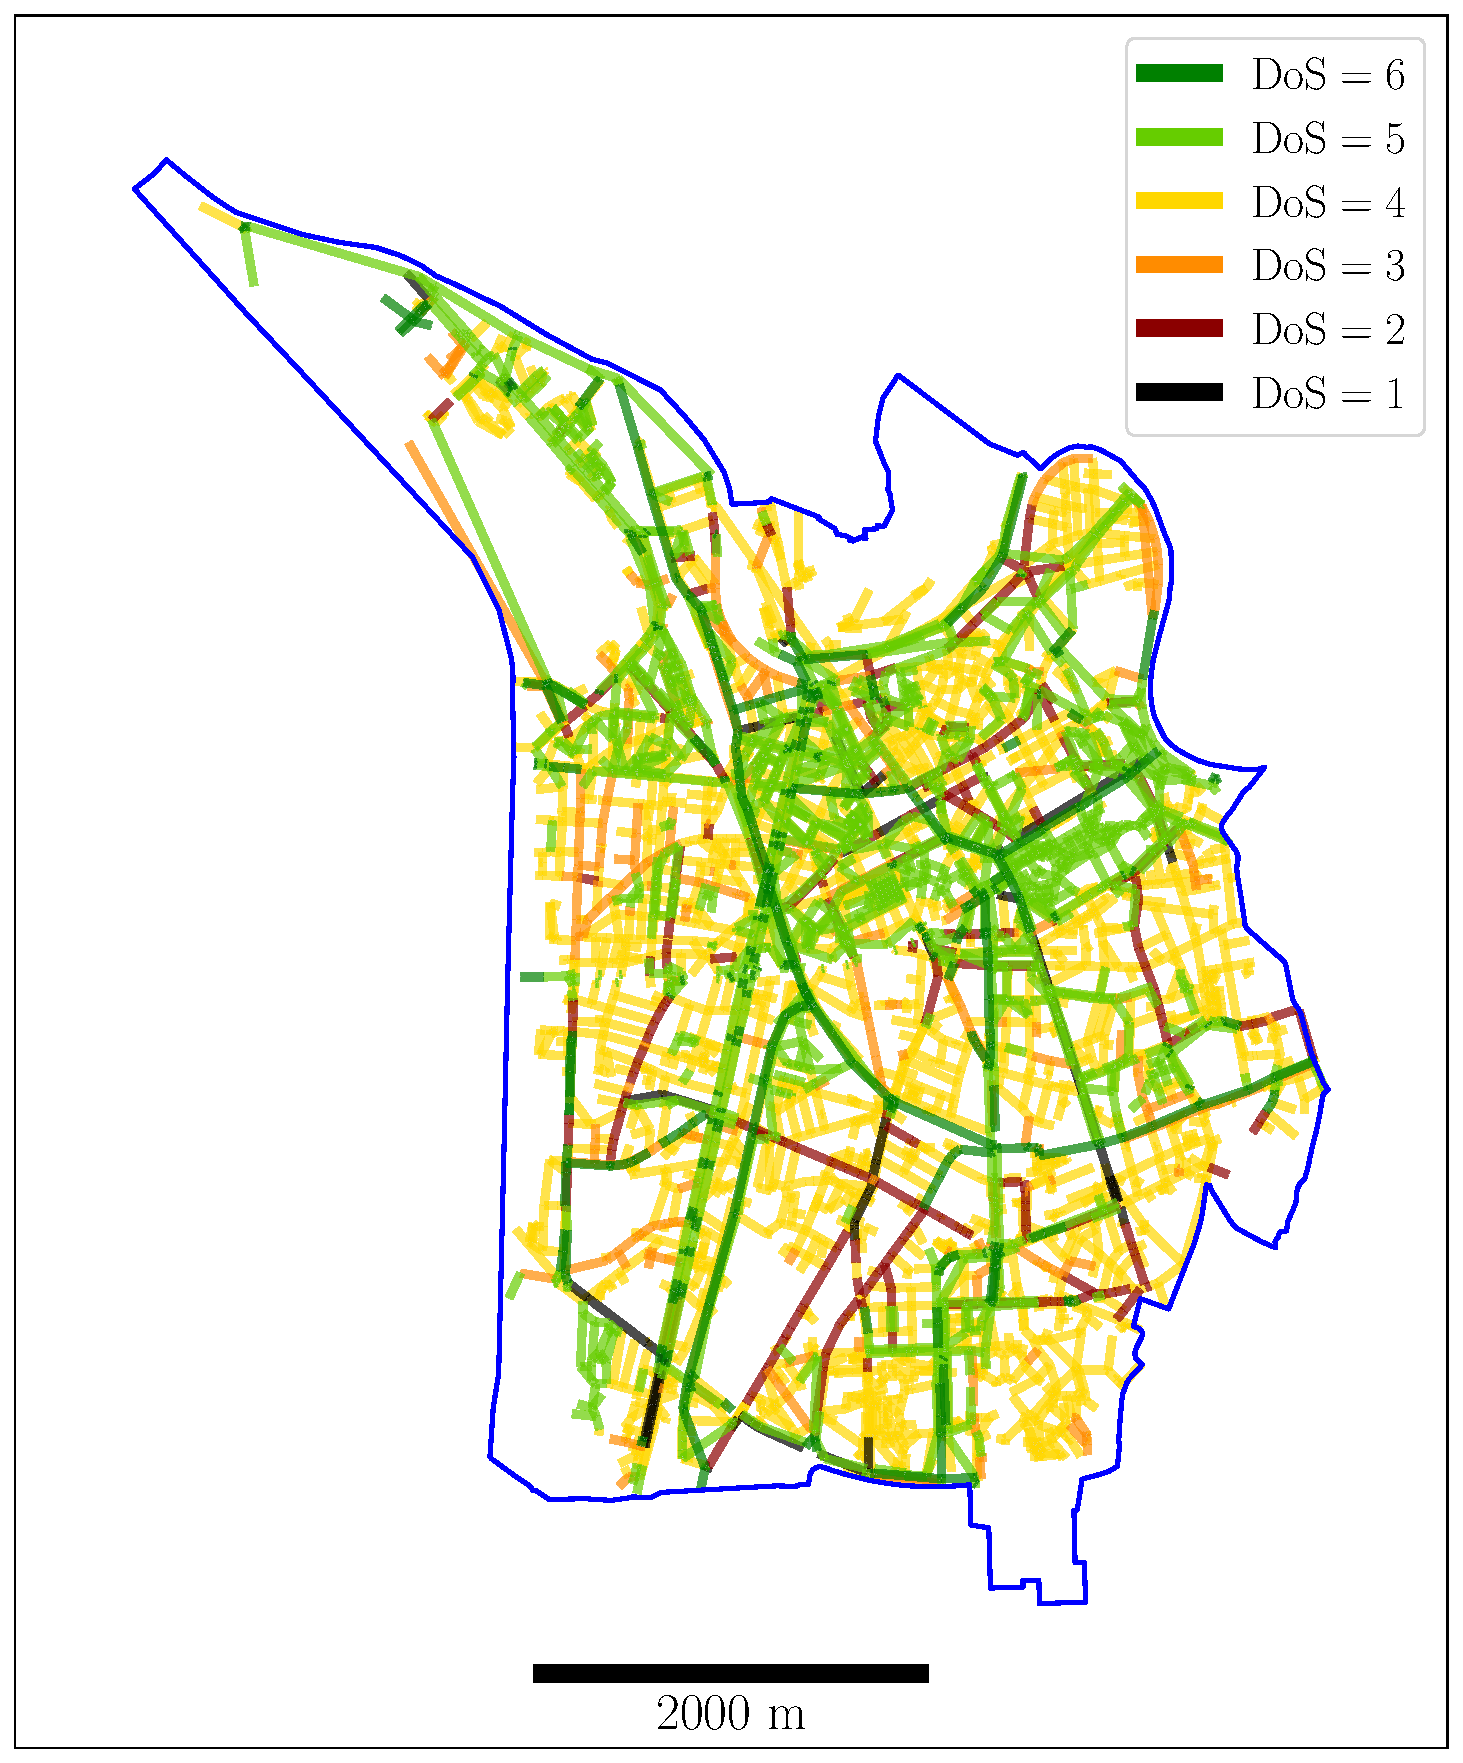
\includegraphics[width=0.48\linewidth]{Images/bikes_network.pdf}
  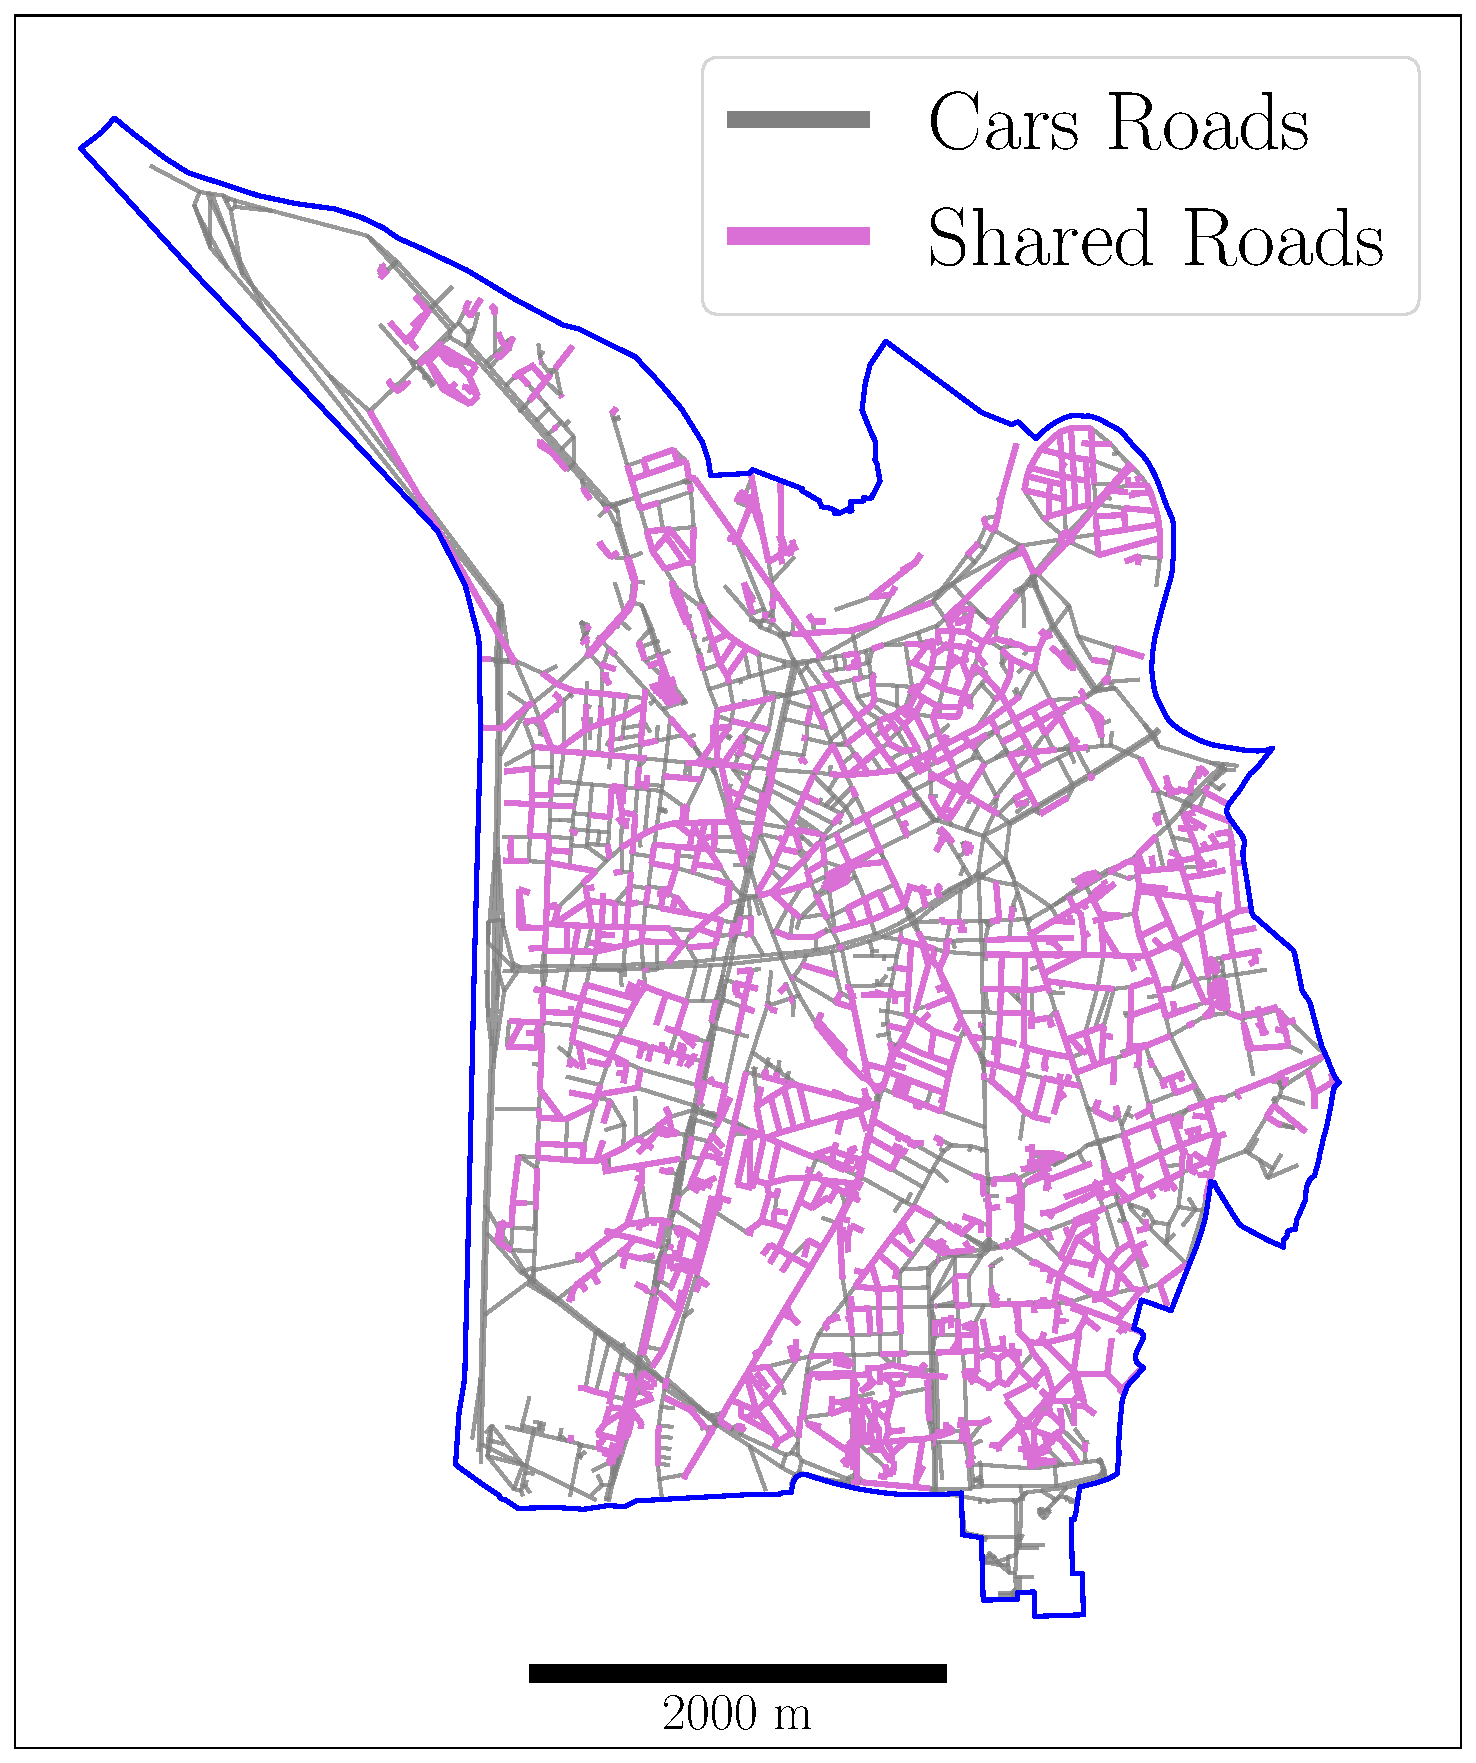
\includegraphics[width=0.48\linewidth]{Images/cars_network.pdf}
  \caption{\footnotesize Multi-modal transportation network of Grenoble, France. \textit{Left:} Cycling infrastructure classified by degree of separation (DoS) of bike lanes, ranging from 1 (least separated) to 6 (fully separated). \textit{Right:} Road network for cars, including links shared with bicycles.}
  \label{multi_network}
\end{figure}


\textit{Organization:} Section~\ref{model_design} describes data sources, bike lane classification, and the overall modeling framework. Section~\ref{solution_algorithm} details the solution algorithm. Section~\ref{case_study} presents the Grenoble case study. Section~\ref{conclusions} concludes with findings and future directions.




\begin{table}[t]
\centering
\vspace{0.2cm}
\begin{tabular}{|>{\centering\arraybackslash}p{0.1\linewidth}|p{0.60
\linewidth}|C{0.15\linewidth}|}
\hline
\textbf{DoS}   & \textbf{Description} & \textbf{AADT (veh/day)} \\
\hline
$6$  & Dedicated bike lanes, fully separated from motor traffic. & 14 400 \\

$5$  & Bike lanes shared with pedestrians, separate from cars. & 16 000 \\ 

$4$  & Mixed-traffic roads (30 km/h) without designated bike lanes. & 960  \\

$3$  & Shared roads with cycling pictograms. & 3 120 \\

$2$  & Roads with painted bike lanes.  & 6 912 \\

$1$  & Unmarked shared car-bike lanes. & 8 448 \\
\hline
\end{tabular}
\caption{\footnotesize The degree of separation (DoS) categorizes bike lane infrastructure based on safety levels. The third column presents annual average daily traffic (AADT) on adjacent car roads, sourced from the GTLVille platform in Grenoble \cite{gtlville2024}.}
\label{dos_table}
\end{table}




% \section{Model Design}
% \label{model_design}
% In this section, we first present the bike lane classification and the graph representation. Next, we introduce the cyclist flow prediction model, the travel time cars model, how the two previous interact between them and the bi-level optimization problem that aims to minimize cyclists' traffic exposure and travel time for cars, directing bike flows toward safer routes. 

% \subsection{Bike Lane  Safety Classification}


% The DoS classification, adapted from an OSM-based platform, categorizes cycling infrastructure based on separation from motor traffic. Table~\ref{dos_table} presents DoS categories, showing that higher-DoS lanes offer greater safety. In this paper, DoS scores are used as weights in the cycling sub-network graph, where an upgrade refers to improving a bike lane from a lower to a higher DoS level. The classification methodology is thoroughly explained in \cite{2024graphbased, jurado2025graph}. Fig.~\ref{multi_network} illustrates these classifications and the cars network in the Grenoble metropolitan area.

% \subsection{Graph Representation}

% The transportation network is modeled as a weighted directed graph (digraph) $\mathcal{G} = (\mathcal{V}, \mathcal{A}, \mathcal{W})$, where $\mathcal{V}$ is the set of nodes (e.g., intersections or endpoints), $\mathcal{A}$ is the set of directed arcs (or links) representing road segments, and $\mathcal{W}$ denotes the corresponding set of edge weights.


% The network comprises two distinct but overlapping layers: the bicycle layer $\mathcal{G}^b = (\mathcal{V}^b, \mathcal{A}^b, \mathcal{W}^b)$ and the car layer $\mathcal{G}^c = (\mathcal{V}^c, \mathcal{A}^c, \mathcal{W}^c)$. Each layer has its own set of nodes, arcs, and weights. Specifically, for each bike arc $a = (u, v) \in \mathcal{A}^b$, the weight $w_a^b$ represents the DoS of $a$, and is symmetric: $w_{(u,v)}^b = w_{(v,u)}^b$. In contrast, car arcs $a \in \mathcal{A}^c$ are uniformly weighted with $w_a^c = 1$, since car travel is modeled without explicitly considering safety concerns.
% Each arc also has an associated geographical length, denoted $d_a^b$ for bicycles and $d_a^c$ for cars, respectively. The full multimodal network satisfies the union relations $\mathcal{V} = \mathcal{V}^b \cup \mathcal{V}^c$ and $\mathcal{A} = \mathcal{A}^b \cup \mathcal{A}^c$. Importantly, the layers may overlap: there can be nodes and arcs that belong simultaneously to both networks, meaning $\mathcal{V}^b \cap \mathcal{V}^c \neq \emptyset$ and $\mathcal{A}^b \cap \mathcal{A}^c \neq \emptyset$.


% Throughout the modeling we use the same notation $a$ for arcs in $\mathcal{A}^b$ and $\mathcal{A}^c$ to simplify expressions, as some arcs belong to both layers ($\mathcal{A}^b \cap \mathcal{A}^c \neq \emptyset$). The layer is indicated by superscripts $b$ or $c$ when needed.

% Finally, let $\mathcal{V}_{\mathcal{O}}^{b}, \mathcal{V}_{\mathcal{D}}^{b} \subseteq \mathcal{V}^{b}$ denote the sets of origin and destination nodes for bicycle trips, and similarly $\mathcal{V}_{\mathcal{O}}^{c}, \mathcal{V}_{\mathcal{D}}^{c}~\subseteq~\mathcal{V}^{c}$ for car trips.


% \subsection{Cyclist Exposure}
% \label{cyclist_exposure}
% For $(u, v) \in \mathcal{V}_{\mathcal{O}}^{b}\times \mathcal{V}_{\mathcal{D}}^{b}$, let $q_{(u,v)}^{b}$ represent the cycling demand between nodes $u$ and $v$. Following the approach in \cite{mesbah2012bilevel}, an all-or-nothing traffic assignment model is considered feasible for bicycles under the assumption of no congestion. In this model, the full demand $q_{(u,v)}^{b}$ is assigned to the shortest path between $u$ and $v$, where distance is measured using a cyclist-specific distance that accounts for the topological characteristics of the bike lane infrastructure. The model estimates flow distribution through betweenness centrality as formalized in \cite{jurado2025improving}, which indicates whether an arc lies on the shortest path between any origin and destination pair and assigns flow accordingly under the all-or-nothing assumption. For an arc $a \in \mathcal{A}^{b}$ in the shortest path $p_{(u,v)}^{b}~=~(a_{1}, \ldots, a_{k})$, $d_{a}^{b}$ is the geographical length; $\measuredangle_{a}^{b}$ represents the angular change (in degrees) along $a$ if it is the first or last arc in the path, or at junctions between consecutive arcs; $s_{a}^{b}$ the slope factor based on the terrain slope $m_{a}^{b}$; and $f_{a}^{b}$ the traffic factor, representing car traffic conditions on roads adjacent to bike lanes, which can significantly impact bike flow on lanes that are shared with car traffic. The cyclist distance $\bar{d}_{(u,v)}^{b}$ between $u$ and $v$, as defined in \cite{cooper2017using}, is given by:
% \begin{equation}
% \label{cyclist_distance}
%     \bar{d}_{(u,v)}^{b} = \sum_{a \in p_{(u,v)}^{b}} \left( d_a^{b} \cdot s_a^{b} \cdot (f_a^{b})^{\rho} \right) +  \sum_{a \in p_{(u,v)}^{b}} \measuredangle_a^{b} \cdot \kappa,
% \end{equation}
% where $\rho > 0$ and $\kappa > 0$ are calibration parameters. The term $f_a^{b} $ represents the traffic exposure factor on arc $a$ and is defined as:
% \begin{equation}
%     f_a^{b} =
%     \begin{cases}
%         \psi \cdot \exp{(\text{AADT}(a))} & \text{if } w_a^{b} < 5, \\
%         \psi \cdot 2.03 & \text{if } w_a^{b} = 5, \\
%         \psi & \text{if } w_a^{b} = 6,
%     \end{cases}
% \end{equation}
% where the parameter $\psi$ is a scaling factor, $w_a^{b}$ is the DoS of the bike lane $a$ and $\text{AADT}(a)$ is the annual average daily traffic  adjacent to bike lanes as in the third column of Table~\ref{dos_table}. According to \cite{cyclerap2024}, the effect of AADT is neutralized if the cycling lane is fully separated from car lanes (i.e., when $\text{DoS} = 5$ or $6$). The factor of 2.03 signifies more than twice the probability of bike crash risk in spaces shared with pedestrians compared to fully separated infrastructure, as identified in \cite{mesimaki2021near}.  Let $p_{(u,v)}^{b}$ denote the shortest path between $u$ and $v$ using the cyclist distance \eqref{cyclist_distance}, and $\phi^{b}_{p_{(u,v)}^{b}}$ the flow assigned to that shortest path. The corresponding flow conservation condition is
% \begin{equation}
% \label{eq_shortest_path}
%     \phi^{b}_{p_{(u,v)}^{b}} = q_{(u,v)}^{b}.
% \end{equation}

% Now, let $\mathbb{I}_{a \in p_{(u,v)}^{b}}$ be a binary indicator that equals 1 if arc $a$ belongs to path $p_{(u,v)}^{b}$, and 0 otherwise. Then,  the total cyclist flow assigned to the the arc $a$, denoted as $\phi_{a}^{b}$, is given by
% \begin{equation}
% \label{eq_flows}
%     \phi_{a}^{b} = \sum_{(u,v) \in \mathcal{V}_{\mathcal{O}}^{b}\times \mathcal{V}_{\mathcal{D}}^{b}} q_{(u,v)}^{b} \cdot \mathbb{I}_{a \in p_{(u,v)}^{b}} \geq 0.
% \end{equation}
% This ensures that the total flow on each arc is the sum of all demands associated with trips traversing it, reflecting the behavior of the betweenness centrality and maintaining network consistency due to the symmetry of the demand matrix. Finally, the cyclist exposure on a given link $a \in \mathcal{A}^{b}$ is computed as the product of the cyclist flow, the traffic exposure factor, and the length of $a$
% \begin{equation}
% \label{arc_exposure}
%     \mathcal{E} = \sum_{a \in \mathcal{A}^{b}} \phi_{a}^{b} \cdot f_a^{b} \cdot d_a^{b},
% \end{equation}
%  this means that exposure is higher on links where more cyclists are present, traffic conditions are more intense, and the segment takes longer to traverse.


\section{Model Design}
\label{model_design}

This section introduces the bike lane classification, the graph-based network model, the cyclist flow prediction, car travel time modeling, and the bi-level optimization that jointly minimizes cyclist exposure and car travel time by steering bike flows toward safer routes.

\subsection{Bike Lane Safety Classification}

We adopt the DoS classification from an OSM-based platform to evaluate cycling infrastructure based on separation from motor traffic. Table~\ref{dos_table} outlines the DoS levels, where higher values indicate safer lanes. In our model, DoS serves as the weight in the bicycle sub-network graph. An upgrade corresponds to moving from a lower to a higher DoS. The classification approach is detailed in \cite{2024graphbased, jurado2025graph}. Figure~\ref{multi_network} shows both the DoS map and the car network in Grenoble.

\subsection{Graph Representation}

The multimodal transport system is modeled as a weighted digraph $\mathcal{G} = (\mathcal{V}, \mathcal{A}, \mathcal{W})$, with nodes $\mathcal{V}$, directed arcs $\mathcal{A}$, and weights $\mathcal{W}$. It consists of two overlapping layers: bicycle $\mathcal{G}^b = (\mathcal{V}^b, \mathcal{A}^b, \mathcal{W}^b)$ and car $\mathcal{G}^c = (\mathcal{V}^c, \mathcal{A}^c, \mathcal{W}^c)$. Each arc $a \in \mathcal{A}^b$ has weight $w_a^b$ equal to its DoS and is symmetric; car arcs use uniform weight $w_a^c = 1$. Geographical lengths are $d_a^b$ and $d_a^c$. Layers may overlap in nodes and arcs, i.e., $\mathcal{V}^b \cap \mathcal{V}^c \neq \emptyset$ and $\mathcal{A}^b \cap \mathcal{A}^c \neq \emptyset$. We use arc notation $a$ across both layers, with superscripts $b$ or $c$ as needed. Origins and destinations are denoted $\mathcal{V}_{\mathcal{O}}^b$, $\mathcal{V}_{\mathcal{D}}^b$ for bikes, and similarly for cars.

\subsection{Cyclist Exposure}
\label{cyclist_exposure}

Let $q_{(u,v)}^b$ be the cycling demand between origin-destination pair $(u,v) \in \mathcal{V}_{\mathcal{O}}^b \times \mathcal{V}_{\mathcal{D}}^b$. Following \cite{mesbah2012bilevel}, we apply an all-or-nothing assignment, allocating demand to the shortest path based on a cyclist-specific distance metric. This metric incorporates infrastructure topology and reflects perceived difficulty and unsafe. Using betweenness centrality \cite{jurado2025improving}, flow is assigned along shortest paths.

For each arc $a \in \mathcal{A}^b$, we define: $d_a^b$: length, $\measuredangle_a^b$: angular change at intersections, $s_a^b$: slope adjustment from terrain gradient $m_a^b$, $f_a^b$: traffic factor due to adjacent car flows.

The cyclist distance $\bar{d}_{(u,v)}^b$ is:
\begin{equation}
\label{cyclist_distance}
    \bar{d}_{(u,v)}^b = \sum_{a \in p_{(u,v)}^b} \left( d_a^b \cdot s_a^b \cdot (f_a^b)^{\rho} \right) + \sum_{a \in p_{(u,v)}^b} \measuredangle_a^b \cdot \kappa,
\end{equation}
with parameters $\rho, \kappa > 0$.

The traffic factor $f_a^b$ depends on DoS and AADT:
\begin{equation}
    f_a^b =
    \begin{cases}
        \psi \cdot \exp(\text{AADT}(a)) & \text{if } w_a^b < 5, \\
        \psi \cdot 2.03 & \text{if } w_a^b = 5, \\
        \psi & \text{if } w_a^b = 6,
    \end{cases}
\end{equation}
where $\psi$ is a scaling constant. As per \cite{cyclerap2024}, AADT effects vanish for DoS 5–6. The 2.03 factor reflects the higher crash risk in shared pedestrian spaces \cite{mesimaki2021near}.

Let $p_{(u,v)}^b$ be the shortest path under Eq. \eqref{cyclist_distance}, with flow $\phi_{p_{(u,v)}^b}^b = q_{(u,v)}^b$. Define a binary indicator $\mathbb{I}_{a \in p_{(u,v)}^b}$ as 1 if arc $a$ is in path $p_{(u,v)}^b$. Then, total arc flow is:
\begin{equation}
\label{eq_flows}
    \phi_a^b = \sum_{(u,v)} q_{(u,v)}^b \cdot \mathbb{I}_{a \in p_{(u,v)}^b} \geq 0.
\end{equation}
Cyclist exposure $\mathcal{E}$ on the network is the sum of arc-level exposures:
\begin{equation}
\label{arc_exposure}
    \mathcal{E} = \sum_{a \in \mathcal{A}^b} \phi_a^b \cdot f_a^b \cdot d_a^b,
\end{equation}
indicating that exposure increases with higher flows, greater traffic influence, and longer travel distance.



% \subsection{Cars Travel Time}

% Similarly to the bicycle network, let $q_{(u,v)}^{c}$ denote the demand between nodes $(u, v) \in \mathcal{V}_{\mathcal{O}}^{c}\times \mathcal{V}_{\mathcal{D}}^{c}$. In contrast to the all-or-nothing traffic assignment, we consider the well-known user equilibrium traffic assignment principle, as described in \cite{maerivoet2005transportation}, which states that no driver can unilaterally reduce their travel time by switching to another route. To compute this equilibrium, it is essential to account for capacity constraints: a reduction in capacity or an increase in travel demand on a link leads to higher travel times, potentially making alternative routes more attractive. To capture this behavior, we use a function that models the travel time experienced by a driver on a given car link $a \in \mathcal{A}^{c}$.
% Let $\phi_a^{c}$ denote the flow on car link $a$, and let $t_a^{c}(\phi_a^{c})$ be the corresponding travel time, which is a function of $\phi_a^{c}$. This travel time is modeled using the Bureau of Public Roads (BPR) function \cite{united1964traffic}, given by:
% \begin{equation}
%     t_a^{c}(\phi_a^{c}) = t_a^0 \left( 1 + \mu \left( \frac{\phi_a^{c}}{\theta_a^{c}} \right)^\sigma \right),
% \end{equation}
% where $t_a^0$ is the free-flow travel time on link $a$, $\theta_a^{c}$ is the maximum flow capacity of the link $a$, and $\mu = 0.15$, $\sigma~=~4$ are calibrated parameters. 

% Now, the question is how to solve the user equilibrium assignment, that is, how to determine the flow $\phi_{a}^{c}$ for each link $a$. To do so, for each pair of nodes $(u, v) \in \mathcal{V}_{\mathcal{O}}^{c}\times \mathcal{V}_{\mathcal{D}}^{c}$, let $\mathcal{P}_{(u,v)}^{c}$ denote the set of possible car paths from node $u$ to node $v$, and let $\phi_{(u,v)}^{p^{c}}$ be the flow assigned to path $p^{c} \in \mathcal{P}_{(u,v)}^{c}$. We impose the following demand constraint:
% \begin{equation}
% \label{t_a_m_1}
%     \sum_{p^{c}\in \mathcal{P}_{(u,v)}^{c}} \phi_{(u,v)}^{p^{c}} = q_{(u,v)}^{c}.
% \end{equation}
% Next, the total flow on each arc $a \in \mathcal{A}^{c}$ is computed by aggregating the path flows in the following way:
% \begin{equation}
% \label{t_a_m_2}
%     \phi_{a}^{c} = \sum_{(u, v) \in \mathcal{V}_{\mathcal{O}}^{c}\times \mathcal{V}_{\mathcal{D}}^{c}} \sum_{p^{c} \in \mathcal{P}_{(u,v)}^{c}} \phi_{(u,v)}^{p^{c}} \cdot \mathbb{I}_{a \in p^{c}} ,
% \end{equation}
% where $\mathbb{I}_{a \in p^{c}}$ is an indicator function equal to $1$ if arc $a$ is part of path $p^{c}$, and $0$ otherwise. Additionally, we require non-negativity of the path and arcs flows
% \begin{align}
%     \label{t_a_m_3_1}
%     \phi_{(u,v)}^{p^{c}} & \geq 0, \quad \forall p^{c} \in \mathcal{P}_{(u,v)}^{c}, \quad \forall (u, v) \in \mathcal{V}_{\mathcal{O}}^{c}\times \mathcal{V}_{\mathcal{D}}^{c}, \\
%     \label{t_a_m_3_2}
%     \phi_{a}^{c} & \geq 0, \quad \forall a \in \mathcal{A}^{c}.
% \end{align}
% The total travel time in the system is then defined as:
% \begin{equation}
%     \mathcal{TTT} = \sum_{a \in \mathcal{A}^{c}} \int_{0}^{\phi_{a}^{c}} t_a^{c}(x) \, \mathrm{d}x.
% \end{equation}
% This is known as the Beckman potential function \cite{beckmann1952lagrangian}, where $\boldsymbol{\phi}^{c} = \left [\phi^{c}_{a} \right ]_{a \in \mathcal{A}^{c}}^\top \in \mathbb{R}_{\geq 0}^{|\mathcal{A}^{c}|}$ denote the vector of cars lanes flows, and the user equilibrium traffic assignment problem is then formulated as the following optimization program:
% \begin{problem}[User Equilibrium Traffic Assignment]
% \label{UE_tp}
% \begin{align*}
% \mathbf{\phi}^{c^{\star}} &\in \mathbb{R}_{\geq 0}^{|\mathcal{A}^{c}|} = \arg\min_{\mathbf{\phi}^{c} \in \mathbb{R}_{\geq 0}^{|\mathcal{A}^{c}|}}  
%    \sum_{a \in \mathcal{A}^{c}} \int_{0}^{\phi_{a}^{c}} t_a^{c}(x) \, \mathrm{d}x  \\
%    \text{s.t. } & \text{\eqref{t_a_m_1}~--~\eqref{t_a_m_3_2}}. \nonumber
% \end{align*}
% \end{problem}
% Then, $\mathbf{\phi}^{c^{\star}} = \left [\phi^{c^{\star}}_{a} \right ]_{a \in \mathcal{A}^{c}}^\top \in \mathbb{R}_{\geq 0}^{|\mathcal{A}^{c}|}$ is the vector of optimal car flows such that no driver can unilaterally reduce their travel time by choosing an alternative route; this corresponds to the user equilibrium condition. The convexity of $\mathcal{TTT}$ and the fact that every minimizer $\boldsymbol{\phi}^{c^{\star}}$ of Problem~1 corresponds to a user equilibrium, i.e., a Nash equilibrium, can be found in \cite{beckman   n1956studies}. In the next section, we proceed to integrate the bicycle traffic exposure model with the car traffic assignment model based on travel time.


\subsection{Cars Travel Time}

Similarly to the bicycle network, let $q_{(u,v)}^{c}$ denote the demand between nodes $(u, v) \in \mathcal{V}_{\mathcal{O}}^{c}\times \mathcal{V}_{\mathcal{D}}^{c}$. Unlike the all-or-nothing assignment, we adopt the UE traffic assignment principle \cite{maerivoet2005transportation}, which assumes that no driver can reduce their travel time by unilaterally changing routes. Capturing this equilibrium requires accounting for capacity constraints: as demand increases or capacity decreases, travel times on a link increase, possibly making alternative paths more appealing. Let $\phi_a^{c}$ denote the car flow on arc $a \in \mathcal{A}^{c}$, and $t_a^{c}(\phi_a^{c})$ be the corresponding travel time. We use the Bureau of Public Roads (BPR) function \cite{united1964traffic}:
\begin{equation}
\label{bpr_function}
    t_a^{c}(\phi_a^{c}) = t_a^0 \left( 1 + \mu \left( \frac{\phi_a^{c}}{\theta_a^{c}} \right)^\sigma \right),
\end{equation}
where $t_a^0$ is the free-flow travel time, $\theta_a^{c}$ is the arc capacity, and $\mu = 0.15$, $\sigma = 4$ are fixed parameters.
To compute equilibrium flows, let $\mathcal{P}_{(u,v)}^{c}$ be the set of car paths between each $(u, v) \in \mathcal{V}_{\mathcal{O}}^{c} \times \mathcal{V}_{\mathcal{D}}^{c}$, and $\phi_{(u,v)}^{p^{c}}$ the path flow on $p^{c}~\in~\mathcal{P}_{(u,v)}^{c}$. The demand constraint reads:
\begin{equation}
\label{t_a_m_1}
    \sum_{p^{c} \in \mathcal{P}_{(u,v)}^{c}} \phi_{(u,v)}^{p^{c}} = q_{(u,v)}^{c}.
\end{equation}
Total arc flow is obtained by summing over path flows:
\begin{equation}
\label{t_a_m_2}
    \phi_{a}^{c} = \sum_{(u,v)} \sum_{p^{c} \in \mathcal{P}_{(u,v)}^{c}} \phi_{(u,v)}^{p^{c}} \cdot \mathbb{I}_{a \in p^{c}},
\end{equation}
where $\mathbb{I}_{a \in p^{c}} = 1$ if arc $a$ is part of path $p^{c}$, and $0$ otherwise. Flows must be non-negative:
\begin{align}
    \label{t_a_m_3_1}
    \phi_{(u,v)}^{p^{c}} & \geq 0, \quad \forall p^{c}, \forall (u,v), \\
    \label{t_a_m_3_2}
    \phi_{a}^{c} & \geq 0, \quad \forall a \in \mathcal{A}^{c}.
\end{align}
The total travel time is defined as the sum over all links of the product of flow and travel time using \cite{beckmann1952lagrangian}:
\begin{equation}
    \mathcal{TTT} = \sum_{a \in \mathcal{A}^{c}} \phi^{c}_{a} \cdot t_a^{c}(\phi_{a}^{c}),
\end{equation}
where $\boldsymbol{\phi}^{c} = \left[\phi_a^c\right]_{a \in \mathcal{A}^c}^\top \in \mathbb{R}_{\geq 0}^{|\mathcal{A}^c|}$. The UE traffic assignment can thus be formulated as:
\begin{problem}[UE Traffic Assignment]
\label{UE_tp}
\begin{align*}
\mathbf{\phi}^{c^{\star}} &\in \mathbb{R}_{\geq 0}^{|\mathcal{A}^{c}|} = \arg\min_{\mathbf{\phi}^{c} \in \mathbb{R}_{\geq 0}^{|\mathcal{A}^{c}|}}  
   \sum_{a \in \mathcal{A}^{c}} \int_{0}^{\phi_{a}^{c}} t_a^{c}(x) \, \mathrm{d}x \\
   \text{s.t. } & \text{\eqref{t_a_m_1}~--~\eqref{t_a_m_3_2}}. \nonumber
\end{align*}
\end{problem}
Then, $\boldsymbol{\phi}^{c^{\star}} = \left[\phi_a^{c^{\star}}\right]_{a \in \mathcal{A}^{c}}^\top$ represents the UE flow assignment, in which no driver can unilaterally reduce their travel time. This flow pattern satisfies the conditions of a Nash equilibrium, as defined in the classical traffic assignment model. The convexity of the total travel time functional 
 $\mathcal{TTT}$ and its connection to user equilibrium are formally established in \cite{beckmann1956studies}. In the next section, we integrate this car traffic assignment model with the cyclist exposure model to form the full bi-level optimization framework.



% \subsection{Interaction Between Cars and New Bike Lanes}

% Upgrading a bike lane may lead to a reduction in the capacity of the adjacent car lane. However, according to \cite{nanayakkara2022safe}, bike lanes that are not fully separated, specifically, those with a DoS less than or equal to 4, do not significantly impact car travel time. In our context, this means that only upgraded bike lanes with a DoS of at least 5 (i.e., fully separated infrastructure) affect car traffic flow. This relationship can be modeled as follows:
% \begin{equation}
% \label{capacity_change}
%     \tilde{\theta}^{c}_{a} = \frac{1}{2} \theta^{c}_{a}, \quad \text{if } \tilde{w}_{a}^{b} \geq 5, \, a \in \mathcal{A}^{c} \cap \mathcal{A}^{b},
% \end{equation}
% where $\tilde{\theta}^{c}_{a}$ denotes the updated car lane capacity on arc $a$, $\theta^{c}_{a}$ is the original capacity, and $\tilde{w}_{a}^{b}$ represents the DoS of the upgraded bike lane, if arc $a$ is shared by both the car and bike networks. As noted in \cite{wiedemann2025bike}, the factor of $\frac{1}{2}$ reflects the reduced space requirement for bicycles compared to cars. This is consistent with common design guidelines, which suggest that a standard bike lane occupies approximately half the width of a car lane, effectively reducing vehicular capacity by about 50\%. At this point, we assume that drivers will not change their chosen routes in response to newly created or upgraded bike lanes. This implies that the optimal car flow $\phi_{a}^{c^{\star}}$ obtained by solving Problem~1 remains unchanged for each $a \in \mathcal{A}^{c}$. However, as discussed previously, the reduction in capacity $\tilde{\theta}^{c}_{a}$ due to the installation of fully separated bike lanes, may increase travel times for cars.  We now introduce the bi-level optimization problem that integrates both the bicycle flow model, which accounts for cyclist exposure, and the fixed car flow model, which may still be affected by capacity changes. 

\subsection{Interaction Between Cars and New Bike Lanes}

Upgrading bike lanes can reduce the capacity of adjacent car lanes. However, as shown in \cite{nanayakkara2022safe}, this effect is negligible for bike lanes with a DoS $\leq 4$. In our setting, only fully separated bike lanes, i.e., those with $\tilde{w}_{a}^{b} \geq 5$, affect car capacity. The capacity reduction is modeled as:
\begin{equation}
\label{capacity_change}
    \tilde{\theta}^{c}_{a} = \frac{1}{2} \theta^{c}_{a}, \quad \text{if } \tilde{w}_{a}^{b} \geq 5, \, a \in \mathcal{A}^{c} \cap \mathcal{A}^{b},
\end{equation}
where $\tilde{\theta}^{c}_{a}$ is the updated car capacity on arc $a$, $\theta^{c}_{a}$ is the original capacity, and $\tilde{w}_{a}^{b}$ is the DoS of the upgraded bike lane on the shared arc. Following \cite{wiedemann2025bike}, the $\frac{1}{2}$ factor reflects that a standard bike lane occupies roughly half the width of a car lane, thus reducing vehicular capacity by 50\%. We assume that drivers do not adjust their routes in response to these changes. Therefore, the car flow vector $\phi^{c^{\star}}$ obtained from Problem~1—computed using the original capacities—remains fixed and represents the pre-upgrade UE traffic assignment, serving as the baseline for our main optimization problem. However, the updated capacities $\tilde{\theta}^{c}_{a}$ in Eq.~\eqref{bpr_function} may still lead to increased travel times. We now introduce the bi-level optimization framework, which integrates the cyclist exposure model with this fixed-flow assumption, while capturing the impact of fully separated bike lane upgrades on car travel times.


\subsection{Optimization Problem}

% Given a fixed budget $B$, our objective is to improve cycling infrastructure by upgrading the DoS on selected road segments. The aim is to minimize cyclists’ average exposure to vehicular traffic, accounting for the distribution of bike flows across the network, while limiting the increase in car travel times.
% As mentioned in the previous subsection, we assume that drivers do not change routes after the bike lanes infrastructure improvements, so the optimal car flows $\phi_{a}^{c^{\star}}$ obtained from solving Problem~1 remain constant. Nevertheless, travel times for cars may increase due to reduced lane capacity, as captured by~equation~\eqref{capacity_change}, and this will be accounted for in the optimization. Each potential upgrade incurs a cost per meter and must respect the budget constraint. We define the following notation:
Given a fixed budget $B$, the objective is to upgrade the cycling infrastructure by increasing the DoS on selected segments, minimizing cyclist exposure while limiting car travel time increases. Car flows $\phi^{c^{\star}}$ remain fixed during optimization, obtained with the pre-upgrade UE assignment from Problem~1. However, travel time penalties from high-DoS upgrades are accounted for via updated capacities following Eq.~\eqref{capacity_change}. Each upgrade incurs a cost and must comply with a global budget constraint.



\begin{itemize}
    \item $\mathbf{w}^{b} = \left [  w_{a}^{b} \right ]_{a \in \mathcal{A}^{b}}^\top \in \mathbb{N}^{|\mathcal{A}^{b}|}$: vector of original DoS values for each arc in the bike network;
    \item $\tilde{\mathbf{w}}^{b} = \left [   \tilde{w}_{a}^{b} \right ]_{a \in \mathcal{A}^{b}}^\top \in \Omega$: vector of decision variables (candidate configuration) representing the upgraded DoS values, where $\Omega$ is the constraint set that defined as $\Omega~=~\left \{ \tilde{w}^{b} \in \mathbb{N}^{|\mathcal{A}^{b}|} \colon w_{a}^{b} \leq \tilde{w}_{a}^{b} \leq 6, \quad \forall a \in\mathcal{A}^{b} \right\};$
\end{itemize}
Additionally, we define the following variables, all normalized between their respective minimum and maximum values:





\begin{table}[h!]
\centering
\vspace{0.2cm}
\begin{tabular}{c|l|c|c}
\hline
\textbf{Symbol} & \textbf{Description} & \textbf{Domain} & \textbf{Unit} \\ \hline
$\phi^{b}_{a}(\tilde{\mathbf{w}}^{b})$ & Flow on arc $a \in \mathcal{A}^{b}$ & $\mathbb{R}_{\geq 0}$ & bike/hr\\
$d_{a}^{b}$ & Length of $a \in \mathcal{A}^{b}$ & $\mathbb{R}_{\geq 0}$ & m \\ 
$\bar{d}_{a}^{b}$ & Cyclist distance of $a \in \mathcal{A}^{b}$ & $\mathbb{R}_{\geq 0}$ & m \\ 
$\mathcal{E}_{a}(\tilde{\mathbf{w}}^{b})$ & Cyclist exposure on  $a \in \mathcal{A}^{b}$ & $\mathbb{R}_{\geq 0}$ & -\\
$\tilde{\theta}^{c}_{a}(\tilde{\mathbf{w}}^{b})$ & Updated car lane capacity &  &  \\
 & on $a \in \mathcal{A}^{c}$ & $\mathbb{R}_{\geq 0}$ & veh/hr \\
$\phi^{c^{\star}}_{a}$ & Pre-upgrade car flow on lane &  &  \\
 & $a \in \mathcal{A}^{c}$  obtained by & & \\
 & solving Problem~1 & $\mathbb{R}_{\geq 0}$ & veh/hr \\
$\pi(w_{a}^{b},\tilde{w}_{a}^{b})$ & Upgrade cost for $a \in \mathcal{A}^{b}$ & $\mathbb{R}_{\geq 0}$ & \$ \\ 
\hline
\end{tabular}
\caption{\footnotesize Abbreviated notation for variables in cycling network model, writing $(\tilde{\mathbf{w}}^{b})$ next to a variable indicates that it is a function of the candidate configuration for bike lane improvements.}
\label{table:notation_summary}
\end{table}
 Now, we present the optimization problem that consists of two interconnected levels:
\begin{problem}[Trade-Off Network-Upgrade]
\label{trade_off_problem}
% \onecolumn
\begin{align}
% & \mathbb{U}_{\text{pper}}: \nonumber \\
% &   \mathbf{w}^{\star}   = \arg\min_{\tilde{\mathbf{w}}^{b} \in \Omega} \;  
%     \epsilon \cdot \left ( \sum_{a \in \mathcal{A}^{b}} \phi_{a}^{b^{\star}}(\tilde{\mathbf{w}}^{b}) \cdot f_a^{b}(\tilde{\mathbf{w}}^{b}) \cdot d_a^{b} \right ) \nonumber \\
%     & + (1-\epsilon) \cdot  \left ( \sum_{a \in \mathcal{A}^{c}} \phi_{a}^{c^{\star}}(\tilde{\mathbf{w}}^{b}) \cdot t_a(\phi_{a}^{c^{\star}}(\tilde{\mathbf{w}}^{b})) \right ) \label{eq:upper} \\
& \mathbb{U}_{\text{pper}}: \nonumber \\
& \mathbf{w}^{\star} = \arg\min_{\tilde{\mathbf{w}}^{b} \in \Omega} \;
\epsilon \cdot \left( \sum_{a \in \mathcal{A}^{b}} \phi_{a}^{b^{\star}}(\tilde{\mathbf{w}}^{b}) \cdot f_a^{b}(\tilde{\mathbf{w}}^{b}) \cdot d_a^{b} \right) \nonumber \\
& + (1-\epsilon) \cdot \left( \sum_{a \in \mathcal{A}^{c}} \phi_{a}^{c^{\star}}\cdot t_a^0 \cdot \left( 1 + \mu \left( \frac{\phi_{a}^{c^{\star}}(\tilde{\mathbf{w}}^{b})}{\tilde{\theta}^{c}_{a}(\tilde{\mathbf{w}}^{b})} \right)^\sigma \right) \right) \label{eq:upper} \\
    & \text{s.t. }   \sum_{a \in \mathcal{A}^{b}} d_{a}^{b} \cdot \pi(w_{a}^{b},\tilde{w}_{a}^{b}) \leq B, \label{eq:budget} \\
& \quad \quad \tilde{\theta}^{c}_{a}(\tilde{\mathbf{w}}^{b}) = \frac{1}{2} \cdot \theta^{c}_{a}  \quad \text{ if } \tilde{w}_{a}^{b} \geq 5, \,  a \in \mathcal{A}^{c} \cap \mathcal{A}^{b}; \label{eq:capacity} \\ 
& \quad \quad \mathbb{L}_{\text{ower}}: \nonumber \\ 
% & \mathbf{\phi}^{b}(\tilde{\mathbf{w}})  = \arg\min_{\mathbf{\phi}^{b} \in \mathbb{R}^{|\mathcal{A}|}_{\geq 0}} \; \bar{\mathbf{d}}^{b}(\tilde{\mathbf{w}})^\top \mathbf{\phi}^{b}  \\
& \quad \quad \boldsymbol{\phi}^{b^{\star}}(\tilde{\mathbf{w}}^{b})  = \arg\min_{\mathbf{\phi}^{b} \in \mathbb{R}^{|\mathcal{A}^{b}|}_{\geq 0}} \; \sum_{a \in \mathcal{A}^{b}} \bar{d}_{a}^{b}(\tilde{\mathbf{w}}^{b}) \cdot \phi_{a}^{b}, \label{eq:lower} \\
% & \quad \quad \text{s.t. }   \phi_{a}^{b}= \sum_{(u,v) \in \mathcal{V}^{b} \times \mathcal{V}^{b}} q_{(u,v)}^{b} \cdot \sigma_{p_{(u,v)}^{b}}(a) \geq 0, \, \forall a \in \mathcal{A}^{b}.   \\
& \quad \quad \text{s.t. } \phi_{a}^{b} = \sum_{(u,v) \in \mathcal{V}_{\mathcal{O}}^{b}\times \mathcal{V}_{\mathcal{D}}^{b}} q_{(u,v)}^{b} \cdot \mathbb{I}_{a \in p_{(u,v)}^{b}} \geq 0, \, \forall a \in \mathcal{A}^{b}.   \nonumber \\
% & \text{as in \eqref{eq_flows}}, \nonumber 
\nonumber
\end{align}
% \twocolumn
\end{problem}
% \begin{equation}
% (1-\epsilon) \cdot  \left ( \sum_{a \in \mathcal{A}^{c}} \phi_{a}^{c^{\star}}(\tilde{\mathbf{w}}^{b}) \cdot t_a(\phi_{a}^{c^{\star}}(\tilde{\mathbf{w}}^{b})) \right )
% \end{equation}
% The \textit{Upper-Level Problem} ($\mathbb{U}_{\text{pper}}$) governs the strategic allocation of upgrades to bicycle infrastructure. Its objective in equation~\eqref{eq:upper} balances two goals: the first term minimizes cyclist exposure to unsafe links, quantified as the product of flow, link-specific traffic factor, and arc length; the second term limits the impact on the total travel time for cars, which may increase due to capacity reductions caused by bike-friendly upgrades ($\text{DoS}\geq 5$). The trade-off between these objectives is controlled by a weight parameter $\epsilon~\in~\left [ 0,1 \right ]$ and is the so-called epsilon-constraint variable. The optimization is subject to a budget constraint equation~\eqref{eq:budget}, capacity reduction rules equation~\eqref{eq:capacity} and the \textit{Lower-Level Problem}~($\mathbb{L}_{\text{ower}}$) in equation~\eqref{eq:lower} that computes the resulting cyclist flows using an all-or-nothing assignment, assuming users choose the shortest paths according to cyclist distance in the upgraded network. The resulting vector of optimal bike lanes flows is denoted by $\boldsymbol{\phi}^{b^{\star}}(\tilde{\mathbf{w}}^{b})~=~\left [\phi^{b^\star}_{a}(\tilde{\mathbf{w}}^{b}) \right ]_{a \in \mathcal{A}^{b}}^\top~\in~\mathbb{R}_{\geq 0}^{|\mathcal{A}^{b}|}$. These flows feed back into the upper-level objective, influencing the cyclist exposure term and thus connecting the two levels of the problem.

% The bi-level optimization in Problem~2 is $\text{NP}\text{-hard}$, as it generalizes the 0-1 knapsack problem where each arc upgrade represents an item with cost $\pi(w_a^{b},\tilde{w}_a^{b})$ and  benefits both  cyclist exposure and traffic flow. The complexity arises from the combinatorial upgrade choices under budget $B$, and the evaluation of cyclist exposure and non-linear car flow effects from changes in $\tilde{\theta}_a^{c}$.
The \textit{Upper-Level Problem} ($\mathbb{U}_{\text{pper}}$) optimizes the distribution of infrastructure upgrades. The first term in~Eq.~\eqref{eq:upper} reduces cyclist exposure by prioritizing links with high flow, traffic, and length. The second term limits additional car travel time due to capacity losses on shared links with  $\text{DoS}~\geq~5$. The trade-off is managed by the weight $\epsilon \in [0,1]$. Constraints Eq.~\eqref{eq:budget} and~\eqref{eq:capacity} enforce the budget limit and car lane capacity reduction rule.
The \textit{Lower-Level Problem} ($\mathbb{L}_{\text{ower}}$) computes bike flows assuming cyclists use shortest paths based on cyclist distance. The resulting flows $\boldsymbol{\phi}^{b^{\star}}(\tilde{\mathbf{w}}^{b})$ influence the upper-level objective via exposure, thus coupling both levels.

Solving Problem~\ref{trade_off_problem} is $\text{NP}$-hard as proved in \cite{jurado2025graph}. It generalizes the knapsack problem, where each arc upgrade is a decision with a cost $\pi(w_{a}^{b},\tilde{w}_{a}^{b})$ and coupled benefits for exposure and car flow, making the problem both combinatorial and nonlinear.


% The complexity derives from the combinatorial selection of upgrades under budget $B$, along with the need to evaluate cyclist exposure responses and non-linear car capacity-flow interactions from $\tilde{\theta}_a^{c}$ modifications.



% The \textit{Upper-Level Problem} ($\mathbb{U}$): Represents strategic infrastructure planning that minimizes both cyclist exposure to car traffic (weighted by arc length, traffic factor, and flow) and car travel time impacts from bike lane upgrades, while respecting the budget $B$. The exposure component prioritizes high-risk arcs, while the travel time term focuses on mitigating capacity reductions from bike lanes with $\text{DoS}~\geq 5$.

% The \textit{Lower-Level Problem} ($\mathbb{L}$): Determines cyclist flow distribution through an AON assignment to shortest paths, where path costs depend on the upper-level DoS decisions. This creates a nested structure where infrastructure upgrades influence route choices, which in turn affect the exposure metrics.




% \section{Solution Algorithm}
% \label{solution_algorithm}
% To tackle the computational complexity of Problem~2 within a practical time frame, we employ the genetic algorithm for bilevel optimization (GA) previously developed in \cite{jurado2025improving}. For completeness, we provide an overview of the algorithm and its main components. 

% The GA algorithm generates and evolves upgrade solutions through selection, crossover, and mutation operations. Each candidate solution $\tilde{\mathbf{w}}^{b}$ is evaluated based on cyclist exposure and cars travel time reduction while respecting budget constraints $B$. During mutation, infeasible solutions exceeding the budget are discarded. The algorithm includes a budget optimization phase that iteratively upgrades arcs with lowest current DoS values when residual budget $\tilde{B}$ remains, ensuring near-complete budget utilization. While not guaranteeing global optimality, this heuristic provides computationally tractable solutions. Algorithm~\ref{pseudocode:SGA} outlines the procedure, where $\Delta_a = \pi(\tilde{w}_a^{b}, w_{\text{DoS}_6})$ denotes the cost to upgrade arc $a \in \mathcal{A}^{b}$ to the highest DoS.

\section{Solution Algorithm}
\label{solution_algorithm}

To solve Problem~\ref{trade_off_problem} efficiently, we adopt the genetic algorithm (GA) from~\cite{jurado2025improving}, which is tailored for bilevel problems. The GA iteratively evolves upgrade configurations $\tilde{\mathbf{w}}^{b}$ using selection, crossover, and mutation, evaluating each solution based on cyclist exposure and car travel time under the budget $B$.

During mutation, solutions exceeding the budget are discarded. To improve budget use, a final optimization step greedily upgrades low-DoS arcs using any remaining budget $\tilde{B}$. While not guaranteeing global optimality, this heuristic provides computationally tractable solutions. Algorithm~\ref{pseudocode:SGA} summarizes the approach. Here, $\Delta_a = \pi(\tilde{w}_a^{b}, w_{\text{DoS}_6})$ is the cost to upgrade arc $a$ to the highest DoS level.

% A description of the procedure is included in Algorithm~\ref{pseudocode:SGA}, where we use the following notation:
% \begin{itemize}
%     \item $\tilde{B}$: Remaining budget after the initial solution $\tilde{\mathbf{w}}^{b}$ has been evaluated.
%     \item $\Delta_a$: The upgrade cost for arc $a \in \mathcal{A}^{b}$, computed as $\pi(\tilde{w}_a^{b}, w_{\text{DoS}_6})$, which is the cost to increase the DoS to its maximum value.
% \end{itemize}
\floatname{algorithm}{Algorithm}
\begin{algorithm}[H]
\caption{GA}
\label{pseudocode:SGA}
\footnotesize
\begin{algorithmic}[1]
\State \textbf{Input:}  $\tilde{\mathbf{w}}^{b}$, $\tilde{B}$
\State \textbf{Output:} Updated arc weights: $\tilde{w}_{a}^{b}$, remaining budget: $\tilde{B}$
\For{$a \in \mathcal{A}^{b}$ sorted by $\text{DoS}(a)$}
    \State Compute upgrade cost: $\Delta_a = \pi(\tilde{w}_a^{b}, w_{\text{DoS}_6})$
    \If{$\tilde{B} \geq \Delta_a$}
        \State Upgrade arc $\tilde{w}_{a}^{b}$ to $w_{\text{DoS}} = 6$.
        \State Update remaining budget: $\tilde{B} \gets \tilde{B} - \Delta_a$
    \EndIf
    \If{$\tilde{B} \leq 0$}
        \State \textbf{Exit}
    \EndIf
\EndFor
\State \textbf{Return:} Updated $\tilde{w}_a^{b}$, remaining $\tilde{B}$
\end{algorithmic}
\end{algorithm}


% \subsubsection{Maximize largest connected component algorithm (MLCC)}

% This algorithm focuses solely on improving cycling network connectivity within budget constraints \cite{2024graphbased}, and serves as a baseline for comparing the SGA’s effectiveness in reducing traffic exposure. It prioritizes upgrading the largest connected component (CC) with the highest DoS to DoS=6. If multiple CCs share this highest DoS, they are connected in order of size using the shortest DoS-path, where bike arcs are weighted by $(7 - w_a^{b})$ to prioritize higher-DoS links. Once a primary high-DoS network is established, other CCs are iteratively linked and upgraded until the budget is exhausted or all edges reach DoS=6. While the algorithm does not explicitly account for cyclist flows, it indirectly improves route choices by favoring high-DoS paths. With polynomial complexity, it efficiently enhances perceived safety and comfort in large cycling networks. Algorithm~\ref{pseudocode:MLCC} outlines the full procedure with the following notation:
% \begin{itemize}
%     \item $\mathcal{C}$: Largest connected sub-network with DoS $=6$.
%     \item $\mathcal{C}_{\gamma}$: Connected component (CC) with DoS level $\gamma \leq 6$.
% \end{itemize}
% \floatname{algorithm}{Algorithm}
% \begin{algorithm}[H]
% \caption{MLCC Algorithm}
% \label{pseudocode:MLCC}
% \footnotesize
% \begin{algorithmic}[1]
% \State \textbf{Input:} Budget $B$, graph $\mathcal{G}$.
% \State \textbf{Output:} Upgraded DoS levels for arcs $\mathcal{A}^{b}$
% \While{$B > 0$ and $\exists$ connected component $\mathcal{C}_{\gamma}$ with DoS $\gamma \leq 6$}
%     \State Find shortest DoS-path between $\mathcal{C}$ and $\mathcal{C}_{\gamma}$
%     \State Upgrade edges along path to DoS $=6$ and update $B$
%     \State Upgrade edges in $C_{\gamma}$ to DoS $=6$ and extend $\mathcal{C}$
% \EndWhile
% \State \textbf{Return:} Final DoS levels for all edges in $\mathcal{A}^{b}$.
% \end{algorithmic}
% \end{algorithm}
% Having presented the methodology and models, we introduce the case study in the next Section.


\section{Grenoble Network Case Study}
\label{case_study}

In this section, we present a case study based in Grenoble, France, and analyze the optimization results obtained using the GA to solve Problem~2. Additionally, we assess the impact of bike lane upgrades on car travel times using a post-upgrade UE traffic assignment.

\subsection{Problem Parameters and Optimal Solution}

To solve the all-or-nothing traffic assignment problem and determine cyclist flows, as described in Section~\ref{cyclist_exposure}, we use parameters recommended in \cite{cooper2017using}, which better suit the model. Specifically, we set $\rho = 0.04$, $\kappa = 0.14$, and $\psi = 0.84$. The slope factor $s_a^{b}$ is defined in Table~\ref{table:slope_factors} as a function of the slope $m_{a}^{b}$, where downhill routes are considered as the reciprocal of the uphill slope factor when traversed in the opposite direction.

\begin{table}[h!]
\vspace{0.2cm}
\centering
\begin{tabular}{c|c|c}
\hline
Slope ($m_a^{b}$) \% & Uphill Factor ($s_a^{b}$) & Downhill Factor ($s_a^{b}$) \\ \hline
$m_a < 2$ & 1.0 & 1.0 \\ 
$2 \leq m_a < 4$ & 1.371 & $1/1.371 \approx 0.729$ \\ 
$4 \leq m_a < 6$ & 2.203 & $1/2.203 \approx 0.454$ \\ 
$m_a \geq 6$ & 4.239 & $1/4.239 \approx 0.236$ \\ \hline
\end{tabular}
\caption{\footnotesize Slope factors for cycling distance calculation}
\label{table:slope_factors}
\end{table}

Let $B = \alpha \cdot B_{\text{max}}$ be the available budget, where $B_{\text{max}}$ is the cost to upgrade the full network to DoS 6 and $\alpha \in [0,1]$. Upgrade costs per meter depend on DoS levels, based on French public estimates~\cite{cerema2024_cost}.

\begin{figure}[t]
\vspace{0.2cm}
  \centering
  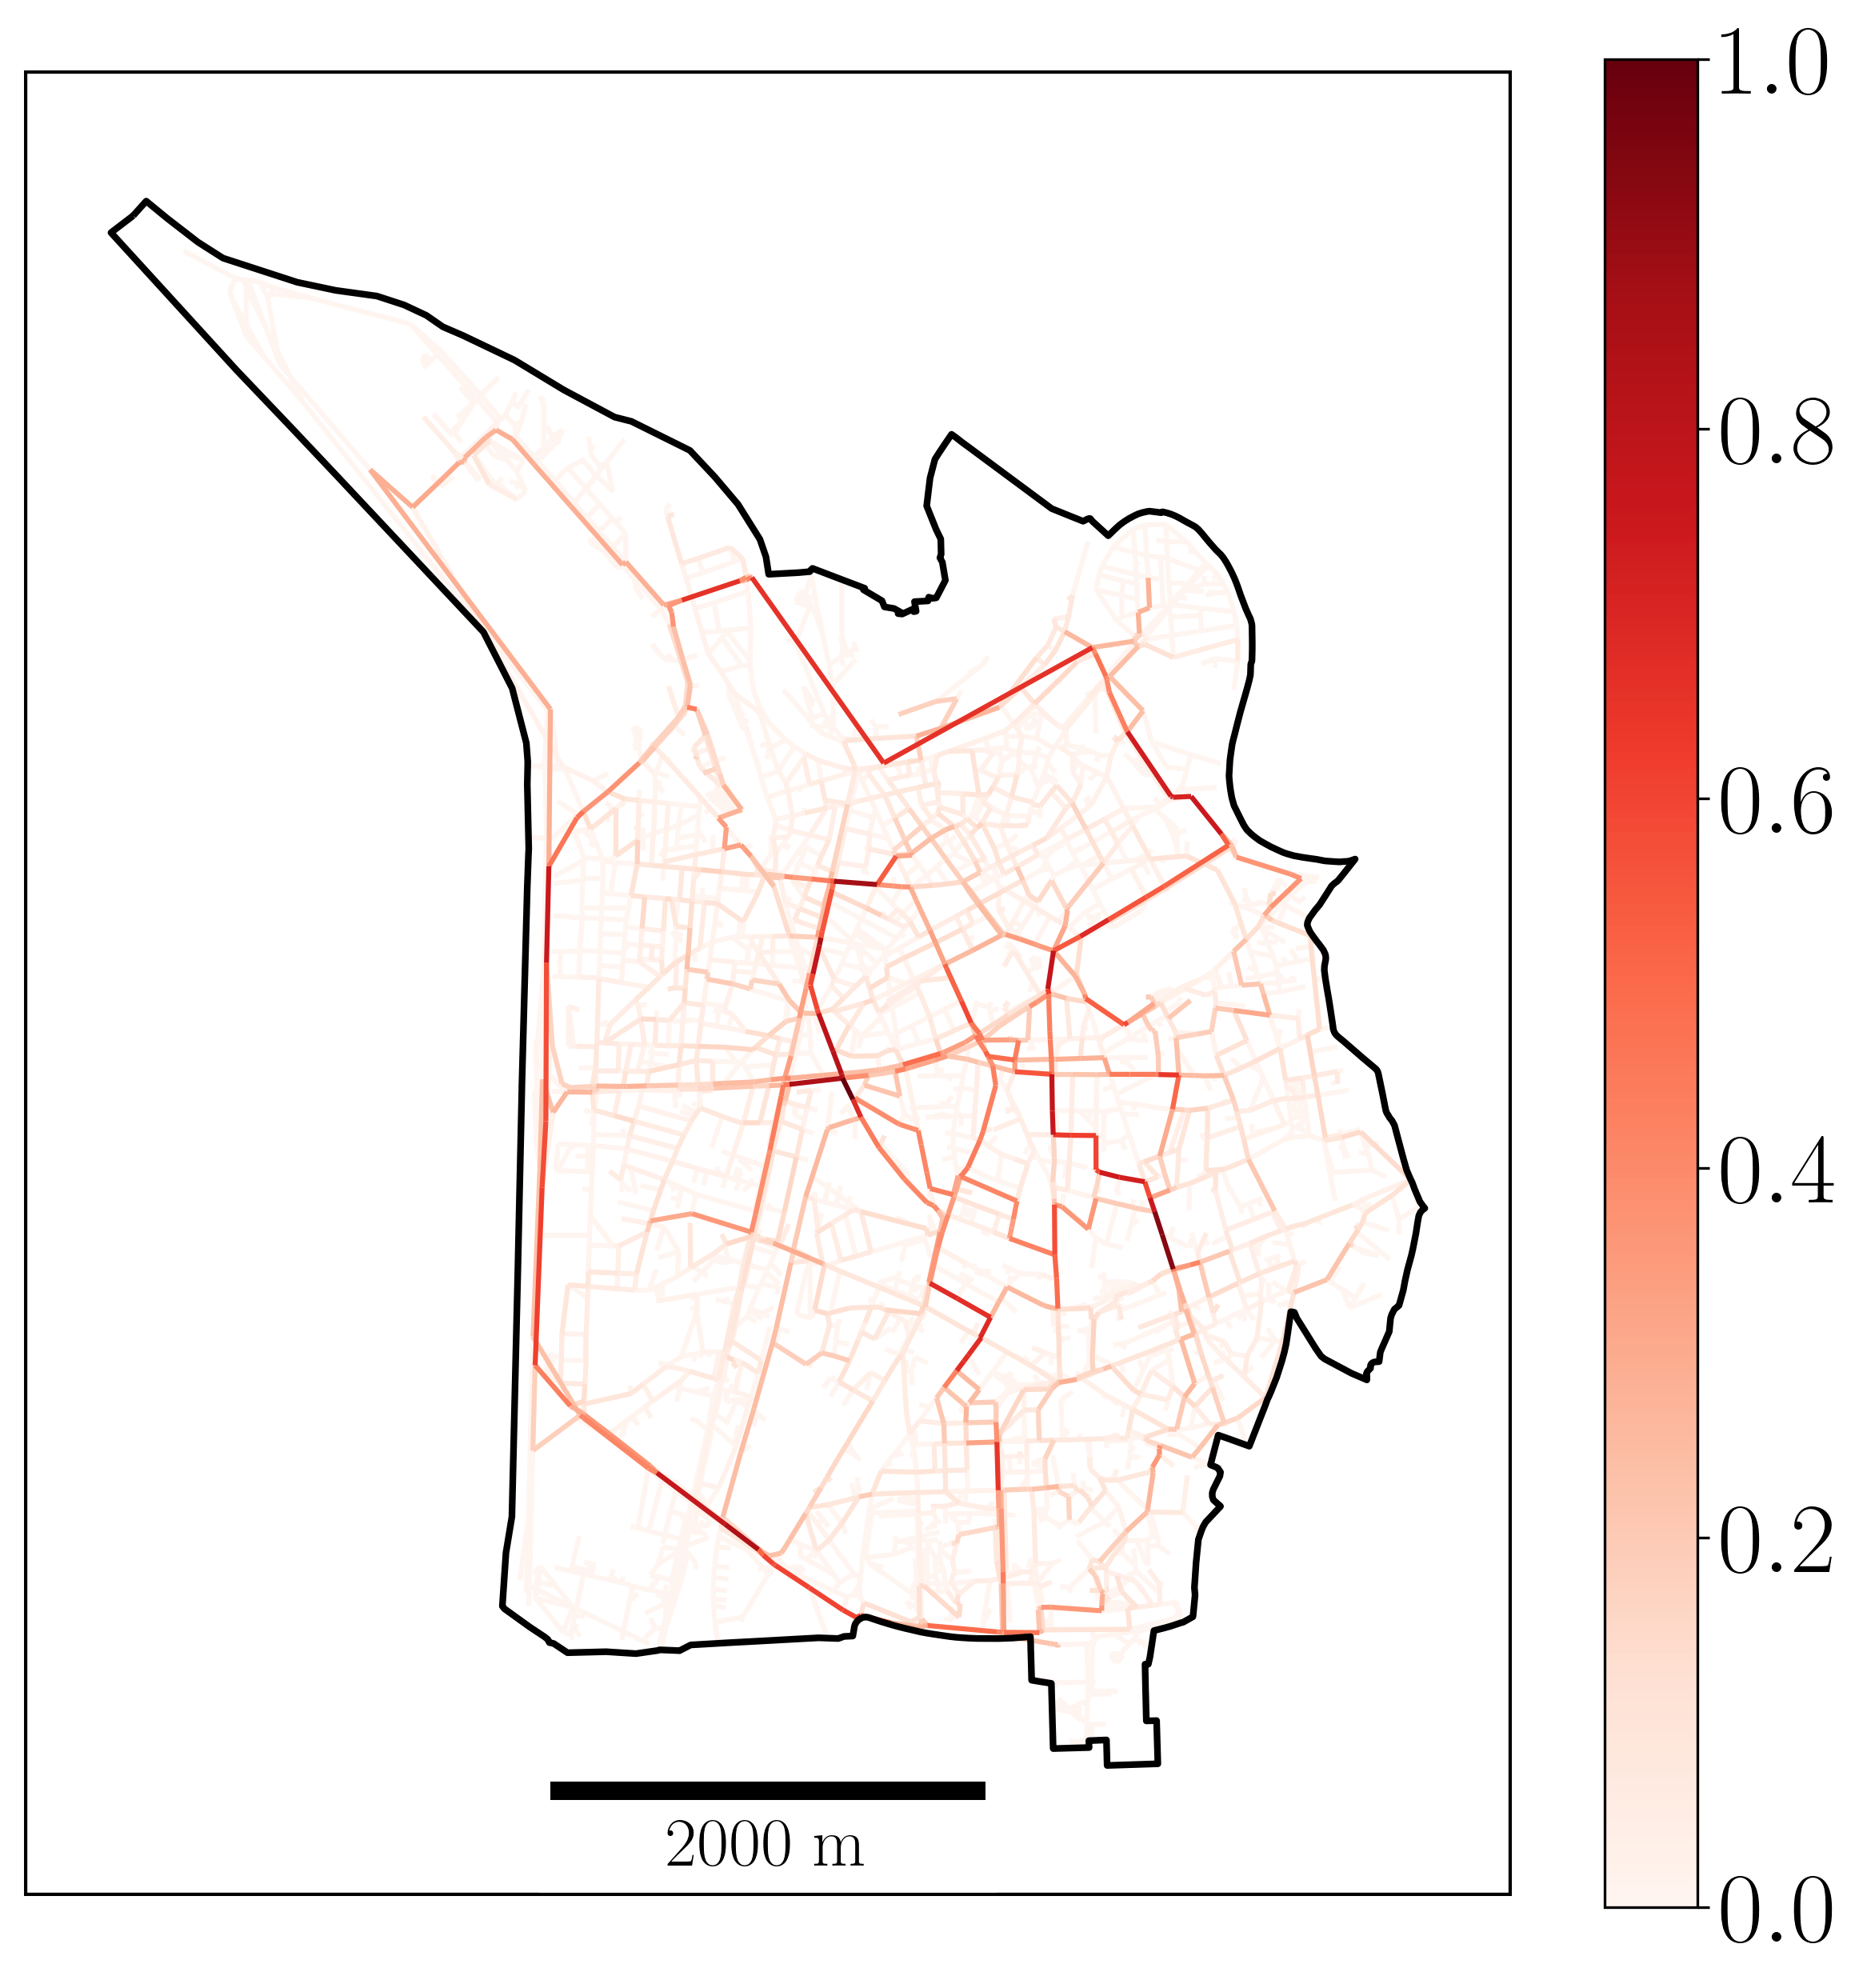
\includegraphics[width=0.58\linewidth]{Images/Grenoble_cars_flows_original.png}
  \caption{\footnotesize Original pre-upgrade UE flows (normalized) obtained by solving Problem~1.}
  \label{original_cars_flows}
\end{figure}
% Now, Fig.~\ref{original_cars_flows} shows the normalized car flows $\mathbf{\phi^{c^{\star}}}$, obtained by solving the user equilibrium traffic assignment for Problem~1 using the deterministic Frank-Wolfe (FW) algorithm \cite{frank1956algorithm, pramesh_kumar_2019_3479554}, which is an iterative method of optimization that successively approximates the nonlinear problem with linear subproblems. These flows are used to solve Problem~2 for three different budgets $\alpha \cdot B_{\max}$ with $\alpha~\in~\Phi~=~\left\{ \frac{1}{3}, \frac{2}{5}, \frac{1}{2} \right\}$, and for ten different values of $\epsilon~\in~\Lambda = \left\{ 0, \frac{1}{10}, \frac{1}{5}, \frac{3}{10}, \frac{2}{5}, \frac{1}{2}, \frac{3}{5}, \frac{7}{10}, \frac{4}{5}, \frac{9}{10}, 1 \right\}$, where $\Lambda$ is called the set of $\epsilon$-constraints. For each $\alpha \in \Phi$, we solve Problem~2 for every $\epsilon \in \Lambda$ and evaluate the resulting set $\left\{ (\epsilon \cdot \mathcal{E}, (1 - \epsilon) \cdot \mathcal{TTT}) \right\}_{\epsilon \in \Lambda}$. The optimal trade-off between cyclist exposure and travel time is defined as the point on the Pareto front with the shortest Euclidean distance to the origin
Fig.~\ref{original_cars_flows} shows the normalized car flows $\phi^{c^{\star}}$ obtained via the Frank-Wolfe algorithm~\cite{frank1956algorithm, pramesh_kumar_2019_3479554} for Problem~1, which represents the baseline pre-upgrade traffic assignment. These are used to solve Problem~2 across three budgets $\alpha \in \Phi = \{ \frac{1}{3}, \frac{2}{5}, \frac{1}{2} \}$ and eleven $\epsilon$-constraint values $\epsilon~\in~\Lambda~=~\{ 0, \frac{1}{10}, \dots, 1 \}$. For each $\alpha$, we evaluate the Pareto set $\left\{ (\epsilon \cdot \mathcal{E}, (1 - \epsilon) \cdot \mathcal{TTT}) \right\}_{\epsilon \in \Lambda}$ and define the optimal trade-off as the closest point to the origin:

\begin{equation}
\label{opt_trade_off}
    \epsilon^{\star}_{\alpha} = \arg\min_{\epsilon \in \Lambda} \sqrt{ \left( \epsilon \cdot \mathcal{E} \right)^2 + \left( (1 - \epsilon) \cdot \mathcal{TTT} \right)^2 }.
\end{equation}
% Fig.~\ref{pareto_front} presents the results of this process. Each point represents a value of $\left( \epsilon \cdot \mathcal{E}, (1 - \epsilon) \cdot \mathcal{TTT} \right)$. When $\epsilon = 0$, the GA focuses entirely on minimizing car travel time, yielding the lowest travel time values. Conversely, when $\epsilon = 1$, the GA focuses entirely on minimizing cyclist exposure, resulting in the highest travel times. The curve corresponding to the budget $\alpha = \frac{1}{2}$ is generally shifted leftward compared to those with lower budgets ($\frac{2}{5}$ and $\frac{1}{3}$), indicating that a higher budget allows more effective upgrades to the cycling network, thereby reducing cyclist exposure. However, this also results in a greater impact on car travel time. On the other hand, the budget $\alpha = \frac{1}{3}$ achieves the least reduction in cyclist exposure but also minimally affects travel time. The optimal trade-off points from equation~\eqref{opt_trade_off} are $\epsilon^{\star}_{\frac{1}{3}}~=~\epsilon^{\star}_{\frac{2}{5}}~=~\frac{3}{10}$ and $\epsilon^{\star}_{\frac{1}{2}} = \frac{4}{10}$. In Fig.~\ref{individual_pareto}, we show the normalized individual results for each $\epsilon \in \Lambda$. As expected, in the original framework, we observe the highest cyclist exposure value of 1 and the lowest travel time value of 0, additionally as observed before, when $\epsilon$ is small, cyclist exposure is high and travel time is low; the opposite is true as $\epsilon$ approaches 1. The optimal $\epsilon^{\star}_{\alpha}$ values are highlighted in red.
Fig.~\ref{pareto_front} displays these trade-offs. When $\epsilon = 0$, travel time is minimized; when $\epsilon = 1$, cyclist exposure is prioritized. Higher budgets (e.g., $\alpha = \frac{1}{2}$) yield lower exposure but slightly higher travel times. The optimal trade-offs occur at $\epsilon^{\star}_{\frac{1}{3}} =  \frac{3}{10}$ and $\epsilon^{\star}_{\frac{2}{5}} =\epsilon^{\star}_{\frac{1}{2}} = \frac{4}{10}$. Fig.~\ref{individual_pareto} shows normalized results for each $\epsilon$, confirming that as $\epsilon$ increases, exposure decreases and travel time rises. Optimal $\epsilon^{\star}_{\alpha}$ points are marked in red.



\begin{figure}[t]
\vspace{0.2cm}
  \centering
  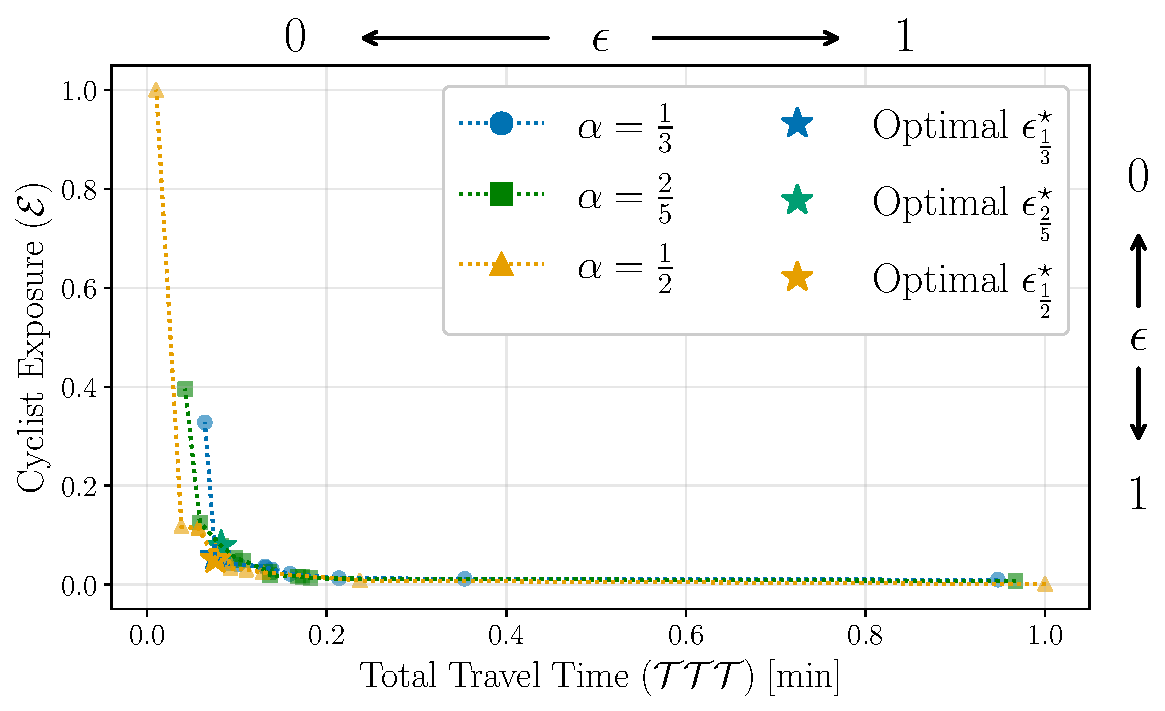
\includegraphics[width=0.8\linewidth]{Images/pareto_front_swapped.pdf} \\


  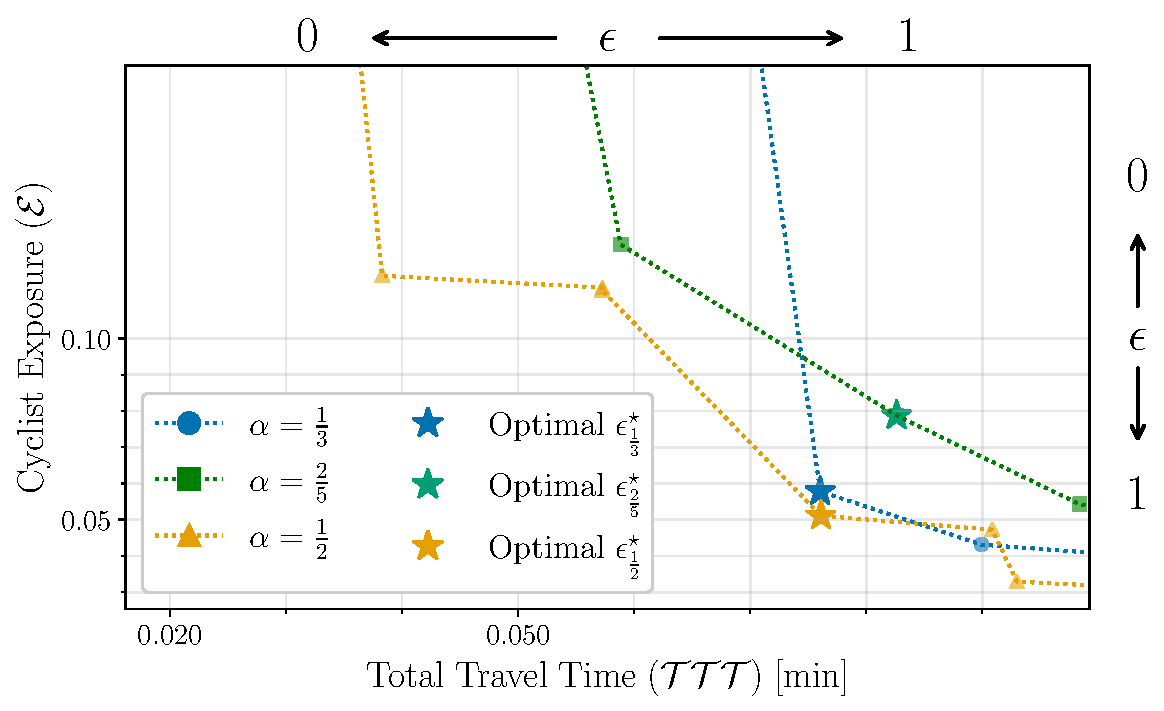
\includegraphics[width=0.8\linewidth]{Images/pareto_front_swapped_zoom.pdf}

  
  \caption{\footnotesize Normalized travel time versus cyclist exposure. The top plot displays the Pareto fronts resulting from the trade-off Problem~2 across different values of $\epsilon \in \Lambda$ and $\alpha \in \Phi$. The bottom plot presents a zoomed-in view focusing on the optimal $\epsilon$-constraint solutions.}
  \label{pareto_front}
\end{figure}


\begin{figure}[t]
\vspace{0.2cm}
  \centering
  \captionsetup[subfigure]{font={footnotesize}, labelfont={footnotesize, bf}, textfont={footnotesize, rm}}

  \subfloat[$\alpha=\frac{1}{3}$]{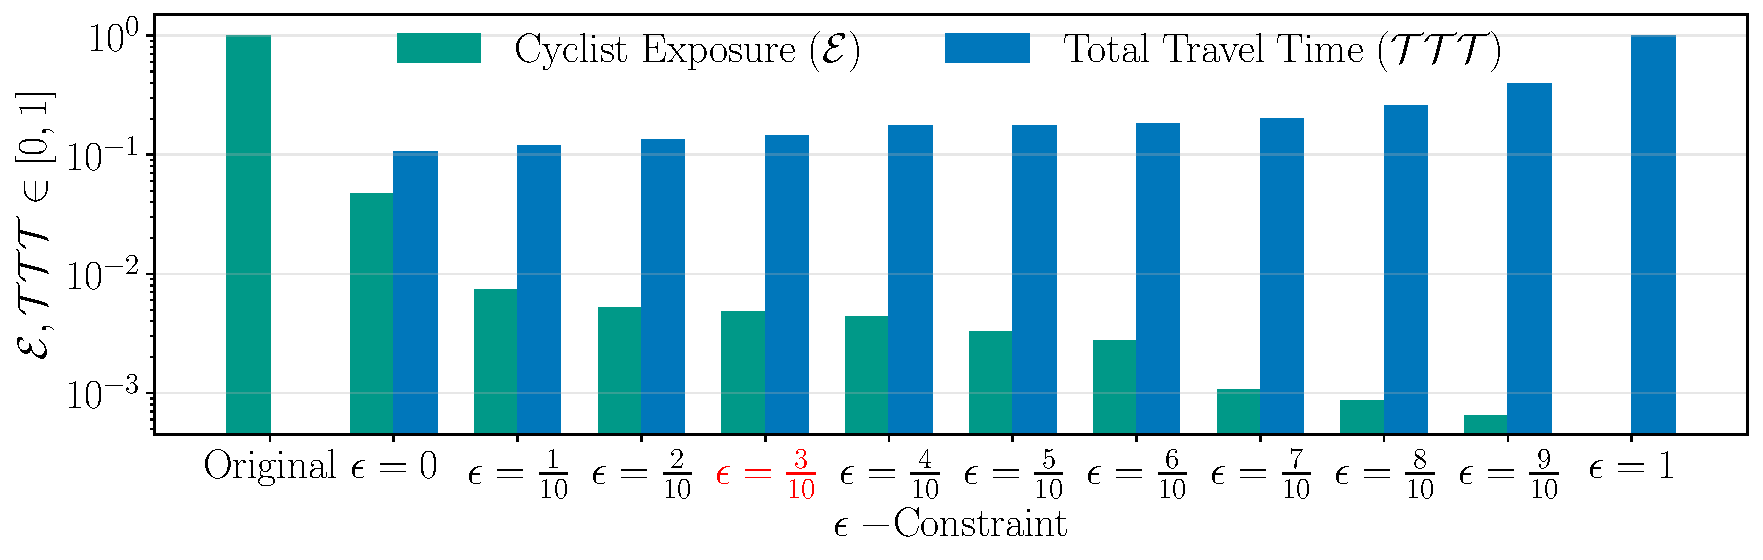
\includegraphics[width=1\linewidth]{Images/exposure_travel_time_comparision_1_3.pdf}}\label{tr_tr_1} \\
  \subfloat[$\alpha=\frac{2}{5}$]{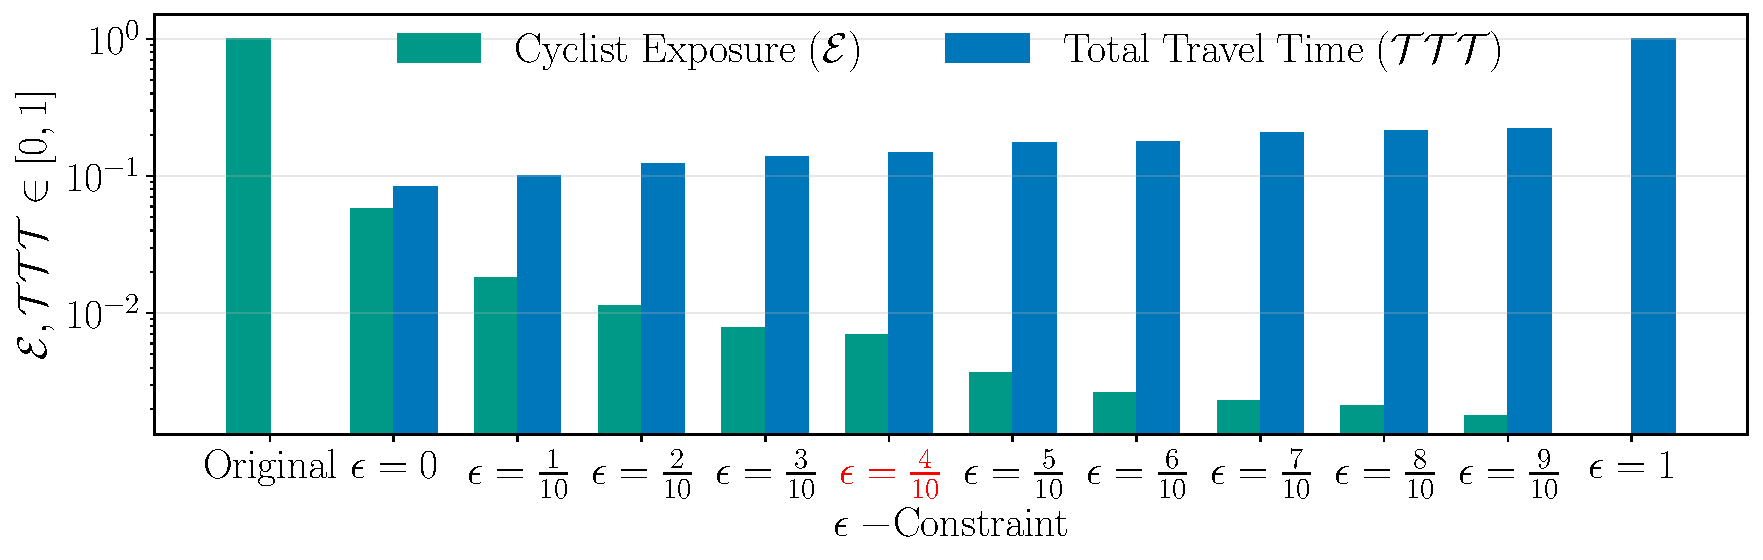
\includegraphics[width=1\linewidth]{Images/exposure_travel_time_comparision_2_5.pdf}}\label{tr_tr_2} \\
  \subfloat[$\alpha=\frac{1}{2}$]{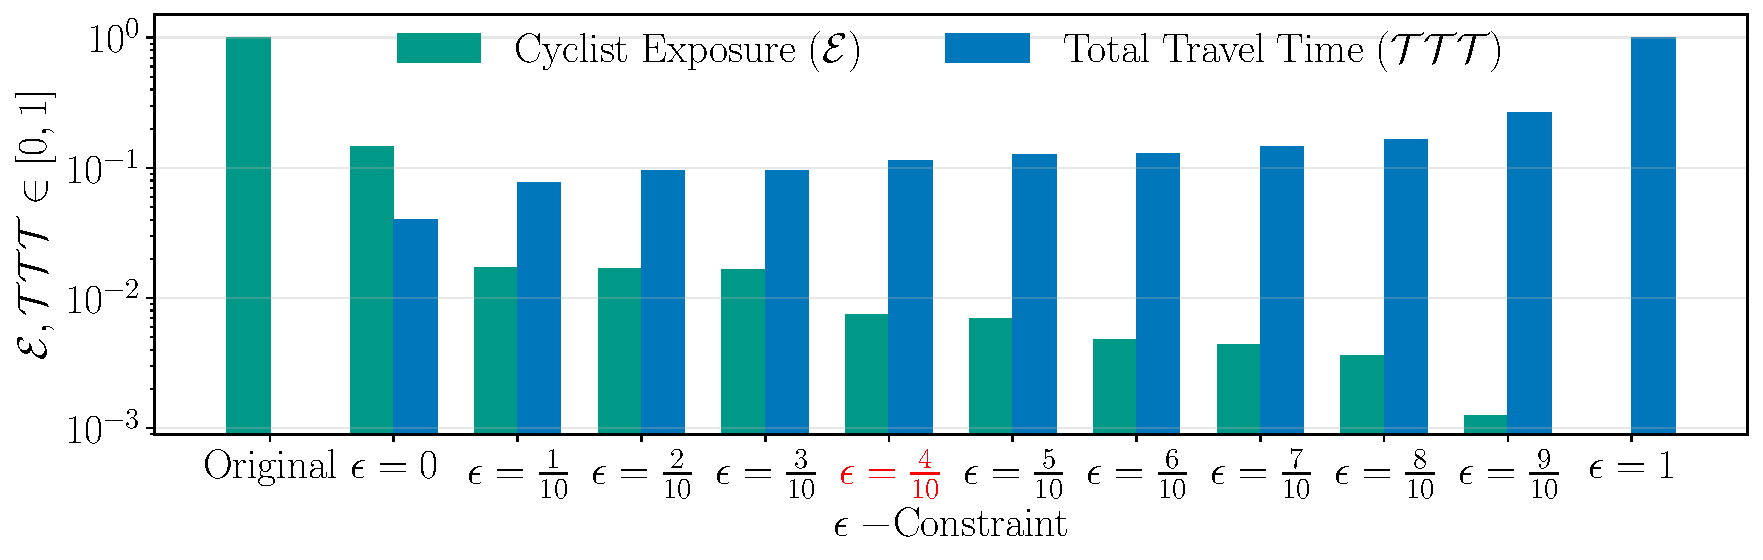
\includegraphics[width=1\linewidth]{Images/exposure_travel_time_comparision_1_2.pdf}}\label{tr_tr_3}
  
  \caption{\footnotesize Normalized cyclist exposure and travel time for each $\epsilon \in \Lambda$ and $\alpha \in \Phi$. In red color are the $\epsilon^{\star}_{\frac{1}{3}}, \epsilon^{\star}_{\frac{2}{5}}$ and $\epsilon^{\star}_{\frac{1}{2}}$ from top to bottom, respectively.}
  \label{individual_pareto}
\end{figure}

% \subsection{Impact on Car Routing Choice and Travel Time}


% As mentioned in the previous subsection, we have identified the optimal trade-off points $\epsilon^{\star}_{\frac{1}{3}}, \epsilon^{\star}_{\frac{2}{5}}$, and $\epsilon^{\star}_{\frac{1}{2}}$ through the GA optimization process. To validate our approach, we assess the impact of the resulting bike lane upgrades on car travel times by comparing two scenarios: the original assumption that drivers retain their routes after upgrades, and a post-upgrade user equilibrium traffic assignment, where drivers are allowed to re-optimize their routes in response to bike lane upgrades that may reduce road capacity, solved using the FW algorithm Fig.~\ref{travel_time_comparison} compares car travel times under the fixed-route assumption in the optimal trade-off points and after the post-upgrade user equilibrium traffic assignment. The results show only a slight increase in travel times after allowing for drivers' route choice re-optimization. The largest normalized percentage difference, observed for $\alpha = \frac{1}{2}$, is only $11.1$\%, corresponding to the scenario with the most extensive bike lane upgrades under the highest budget. This suggests that the impact of the upgrades on car traffic remains limited. Further evidence can be seen in Fig.~\ref{bike_network_evolution}~(a)–(c) where the bike network upgrades (as compared to the current network configuration illustrated in  Fig.~\ref{multi_network}) reveal targeted improvements along arcs critical for cyclist safety, prioritizing segments with high cyclist exposure typically near central urban areas or major corridors. Under lower budgets as $\alpha=\frac{1}{3}$, investments focus on specific high-impact segments where safety gains are most cost-effective. In contrast, higher budgets as $\alpha=\frac{1}{2}$ allow broader, though sometimes discontinuous, coverage, often along key routes likely to form critical paths in the cycling network. Post-upgrade user equilibrium car flows in Fig.~\ref{bike_network_evolution}~(d)–(f) remain qualitatively similar to the original flow pattern in Fig.~\ref{original_cars_flows}, confirming minimal disruption to vehicular traffic. Nevertheless, traffic redistributions are observed: for example in Fig.~\ref{bike_network_evolution}~(f), central segments display notable changes in car flow, with colored lanes highlighting the areas of greatest absolute percentage variation. Adjacent routes respond by absorbing or releasing traffic, reflecting a user equilibrium dynamic in which drivers adjust routes to maintain efficient travel times. However, these adjustments are generally moderate, with average flow changes ranging from 20\% to 30\%. Additionally, the 
% $\alpha=\frac{1}{2}$ scenario in Fig.~\ref{bike_network_evolution}~(f) shows marginally more flow dispersion compared to lower-budget cases, consistent with its greater network modifications. However, these shifts result in only minor increases in travel time at the network level as was discussed in Fig.~\ref{travel_time_comparison}, underscoring that well-targeted cycling upgrades can enhance safety without sacrificing vehicular traffic performance.

\subsection{Impact on Car Routing Choice and Travel Time}

To assess the impact of upgrades at $\epsilon^{\star}_{\alpha}$, we compare the UE traffic assignment computed on the pre-upgrade network (i.e., assuming drivers maintain their original routes) with the post-upgrade UE assignment, where drivers re-optimize their routes in response to updated capacities. Using the Frank-Wolfe method, Fig.~\ref{travel_time_comparison} shows that even after route re-optimization, travel times increase only slightly (maximum 11.1\% for $\alpha~=~\frac{1}{2}$), indicating limited disruption to car traffic.

Fig.~\ref{bike_network_evolution}~(a)–(c) shows bike lane improvements focus on high-impact segments, especially with lower budgets. Higher budgets allow for greater, but less continuous expansion. Car flows in Fig.~\ref{bike_network_evolution}~(d)–(f) remain similar to the original (Fig.~\ref{original_cars_flows}), though some central segments show notable flow changes (e.g., Fig.~\ref{bike_network_evolution}~(f)). These localized redistributions reflect moderate adjustments in user equilibrium, with most flow changes between 20–30\%. The broader dispersion under $\alpha = \frac{1}{2}$ aligns with its more extensive upgrades. Overall, these shifts result in modest travel time increases, confirming that targeted upgrades can enhance cyclist safety with minimal impact on vehicular efficiency.





% \begin{figure}[t]
% \vspace{0.2cm}
%   \centering
%   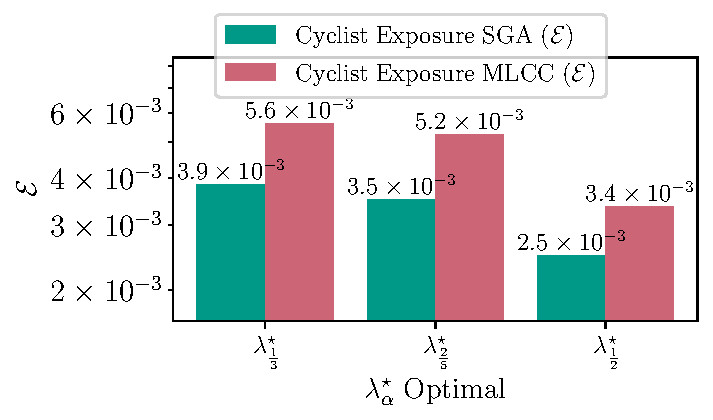
\includegraphics[width=1\linewidth]{Images/cyclist_exposure_comparision.pdf}
%   \caption{\footnotesize Comparison of cyclist exposure between the SGA algorithm using optimal values $\epsilon_{\alpha}^{\star}$ and the MLCC algorithm under the same budget $\alpha~\cdot~B_{\max}$, for each $\alpha \in \Phi$.}
%   \label{cyclist_exposure_c}
% \end{figure}

\begin{figure}[t]
\vspace{0.2cm}
  \centering
  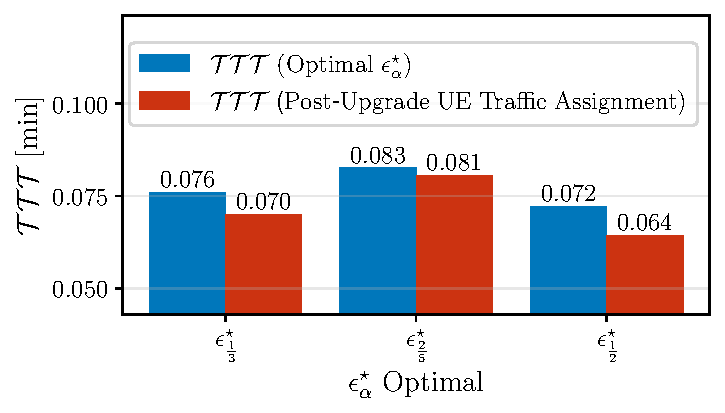
\includegraphics[width=0.7\linewidth]{Images/cars_flows_comparision.pdf}
  \caption{\footnotesize Comparison of car travel times at the optimal trade-off points $\epsilon_{\alpha}^{\star}$, with post-upgrade UE traffic assignment after bike lane upgrades at these locations.}
  \label{travel_time_comparison}
\end{figure}


\begin{figure*}[t]
\vspace{0.2cm}
  \centering
  \captionsetup[subfigure]{font={footnotesize}, labelfont={footnotesize, bf}, textfont={footnotesize, rm}}

  \subfloat[Optimal upgrade for $\epsilon^{\star}_{\frac{1}{3}}$]{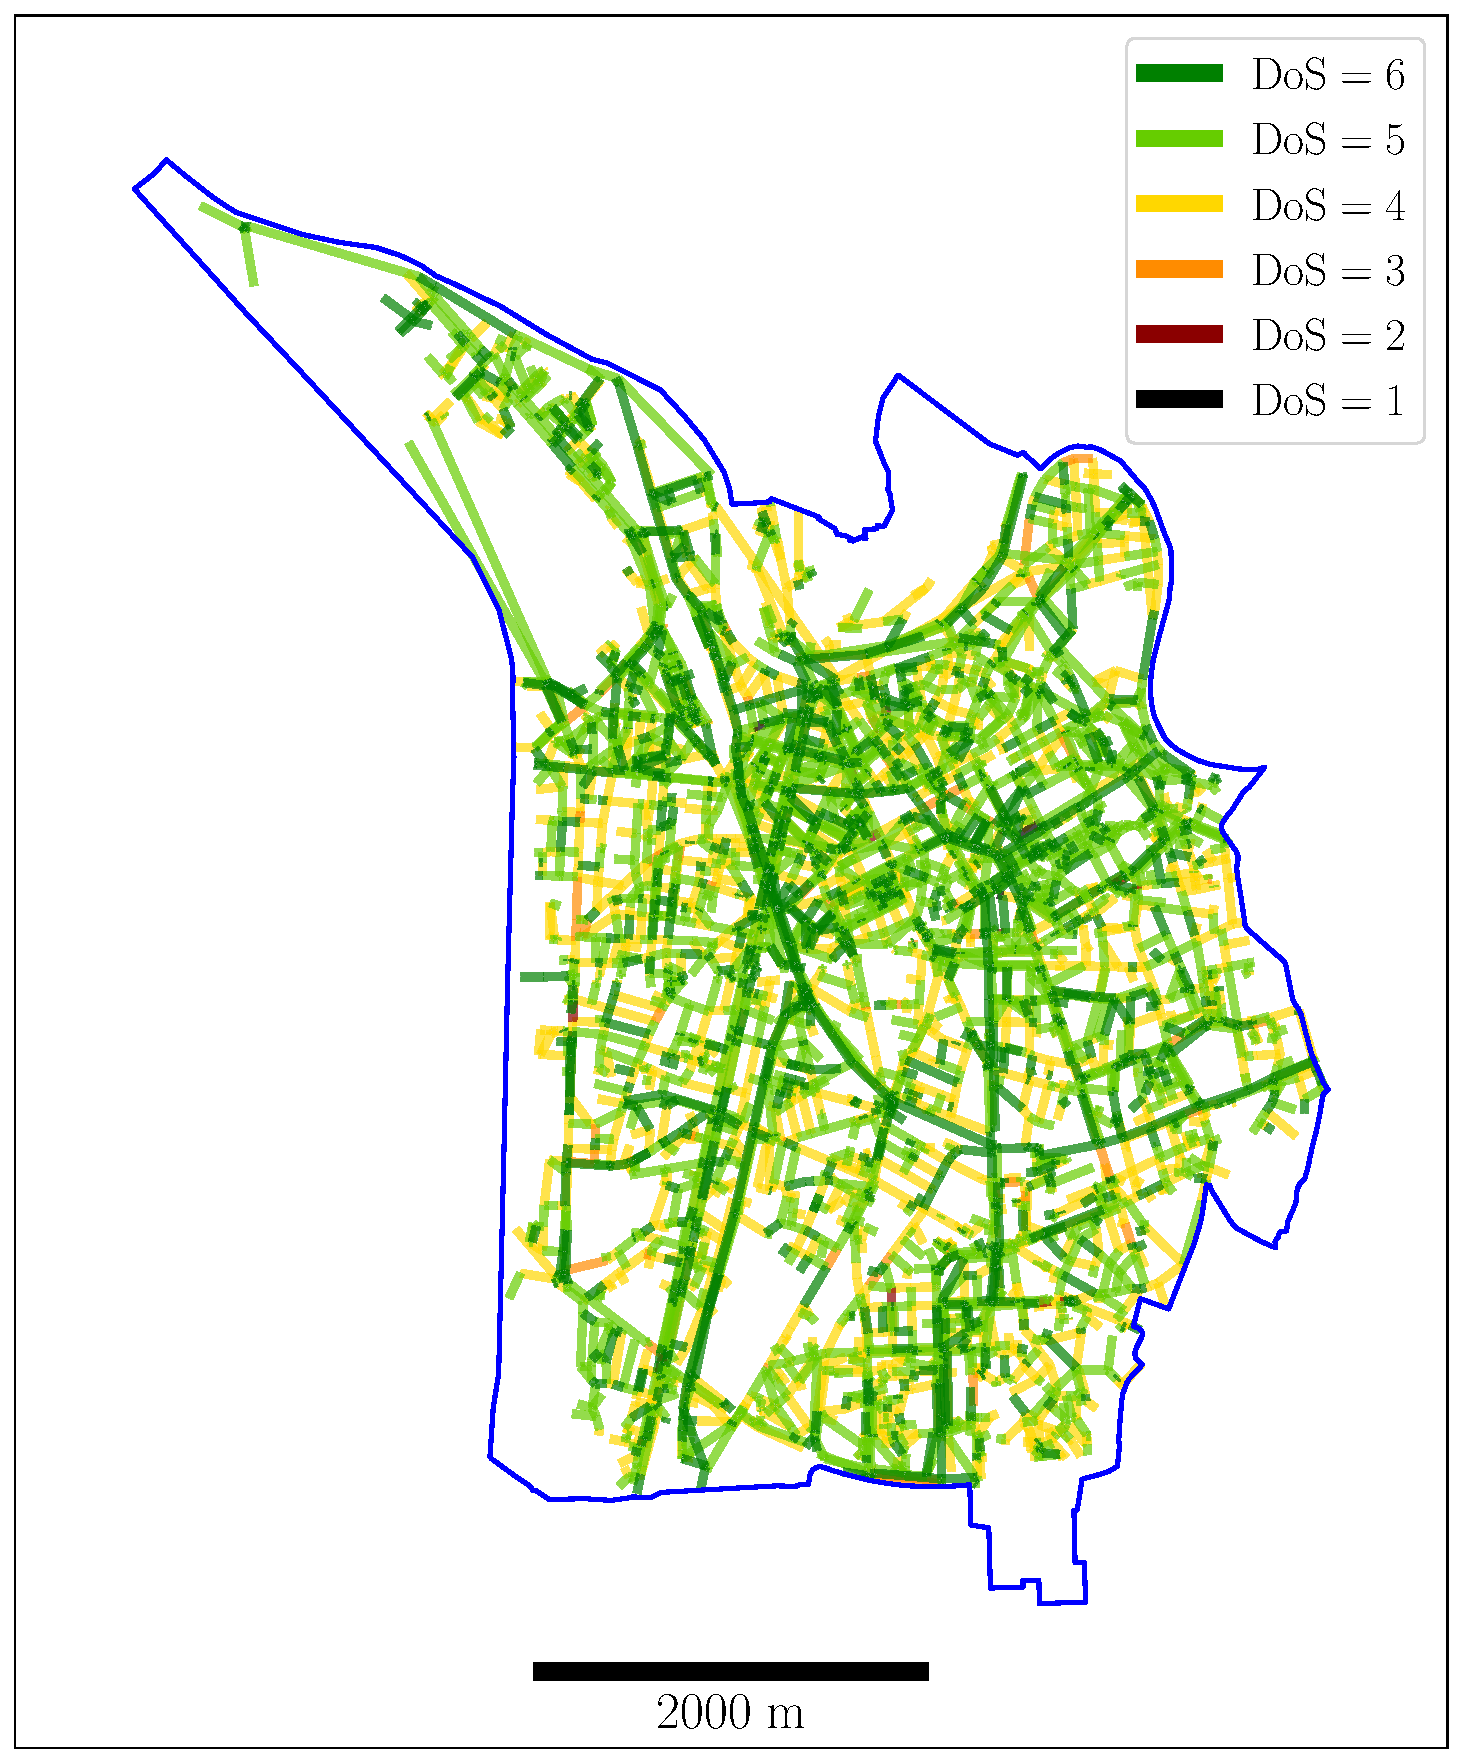
\includegraphics[width=0.25\linewidth]{Images/bike_network_sga_1_3.pdf}}\label{sga_1} \hspace{0.09\linewidth}
  \subfloat[Optimal upgrade for $\epsilon^{\star}_{\frac{2}{5}}$]{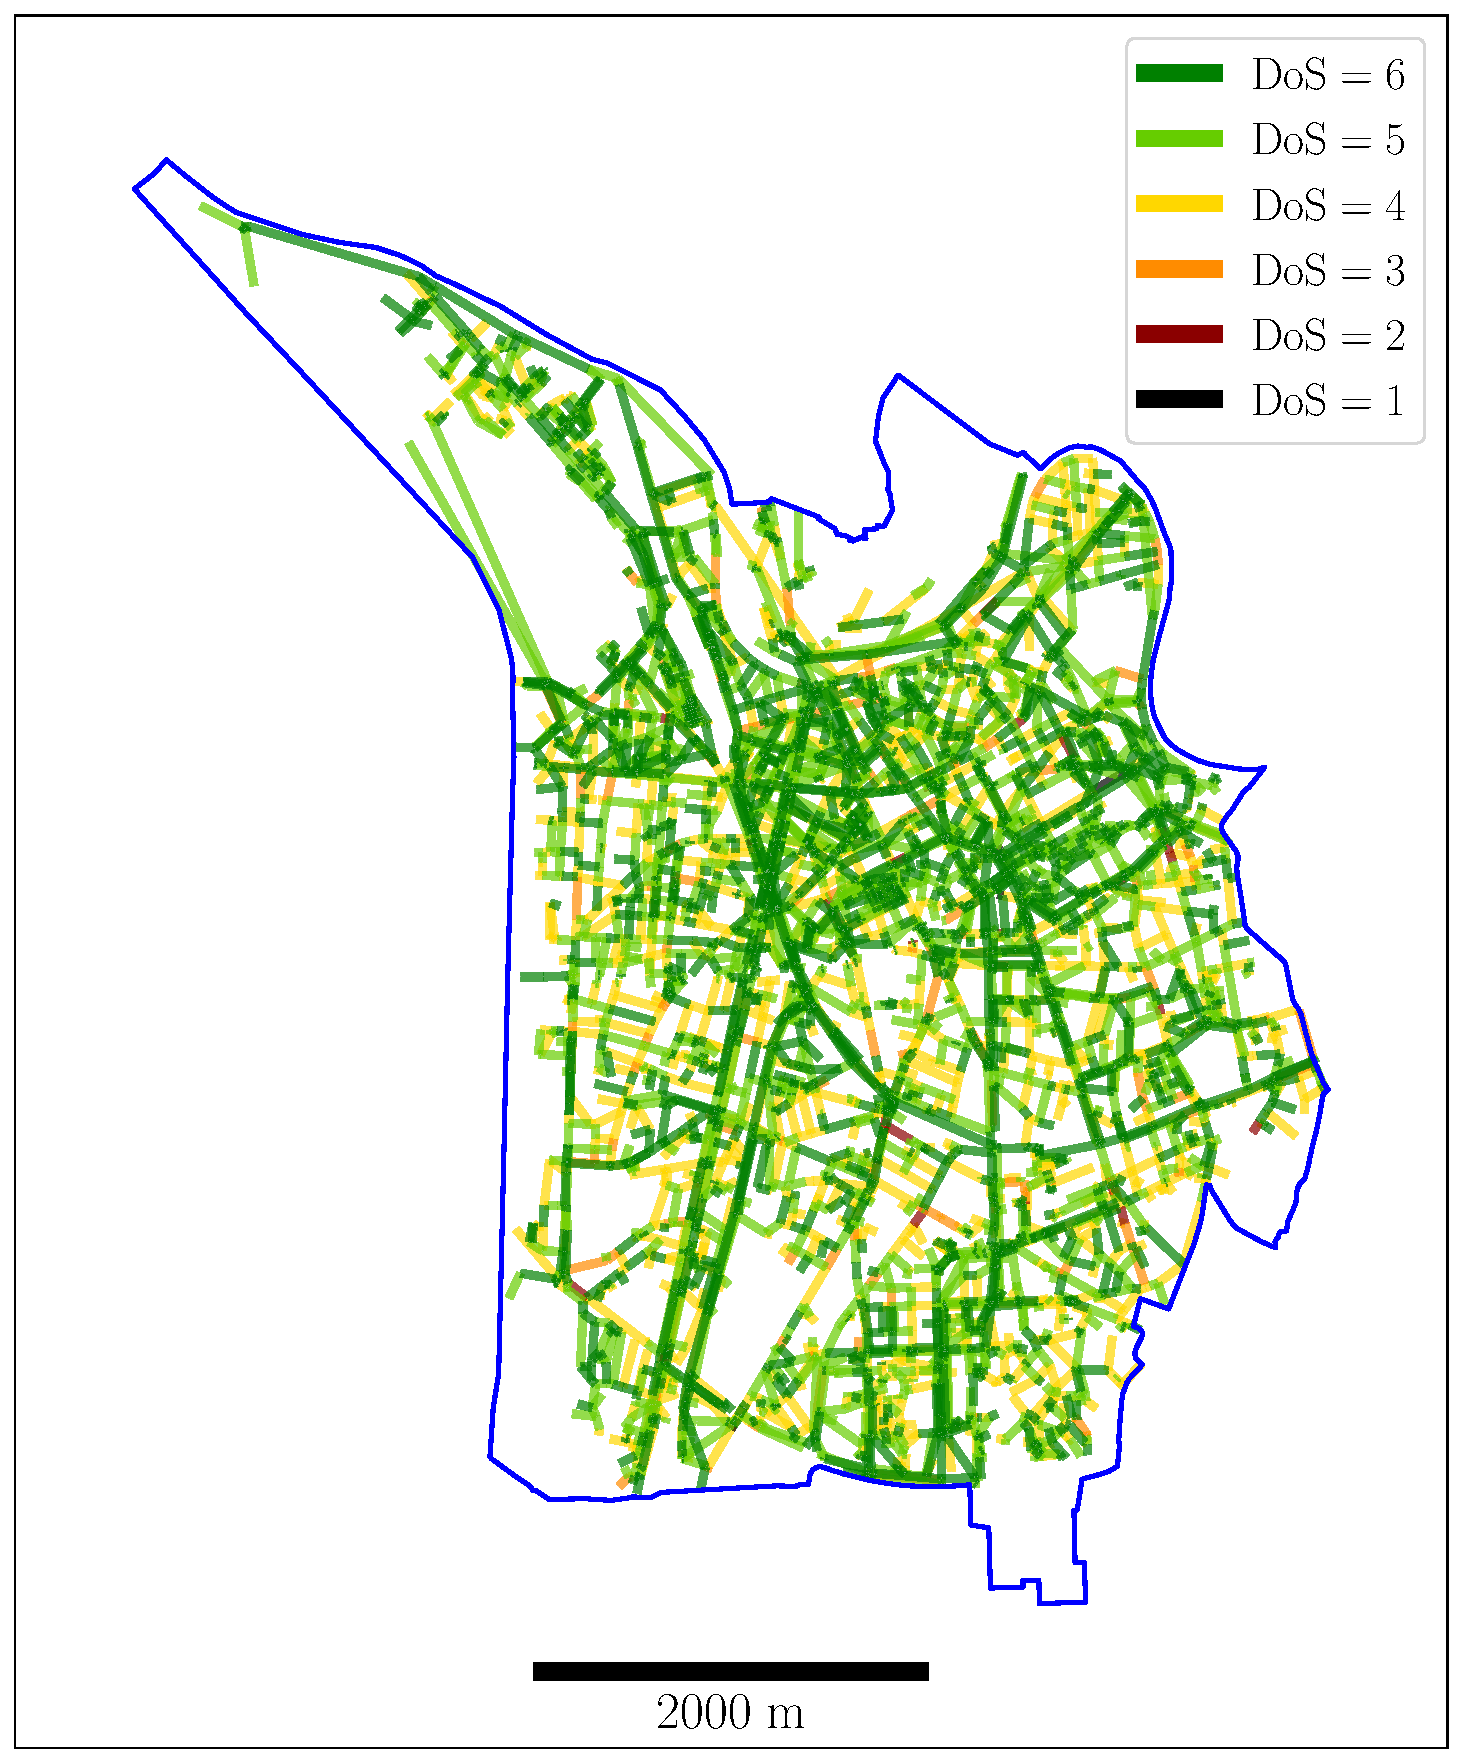
\includegraphics[width=0.25\linewidth]{Images/bike_network_sga_2_5.pdf}}\label{sga_2} \hspace{0.07\linewidth}
  \subfloat[Optimal upgrade for $\epsilon^{\star}_{\frac{1}{2}}$]{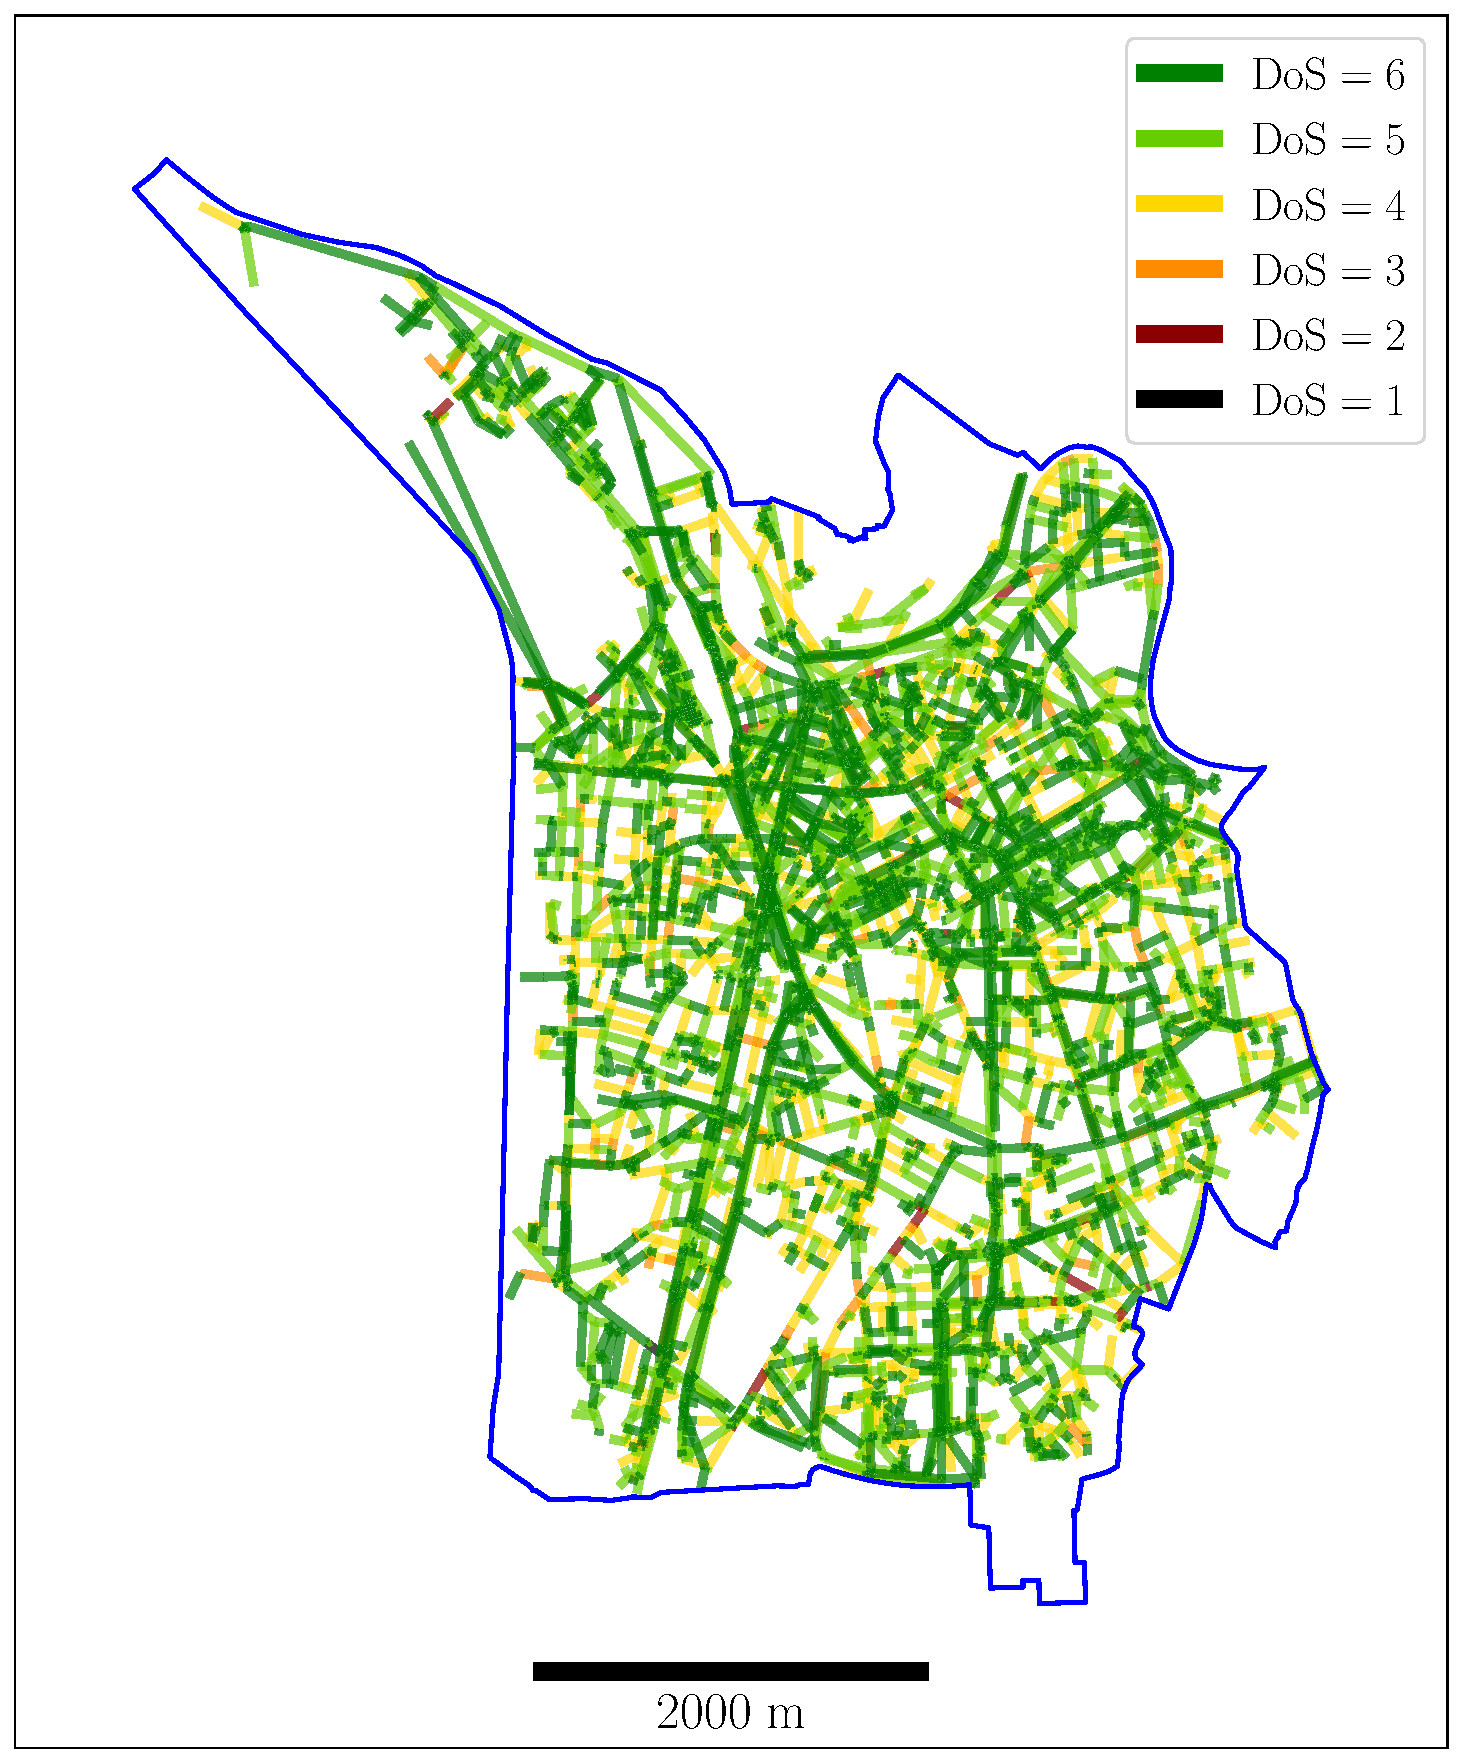
\includegraphics[width=0.25\linewidth]{Images/bike_network_sga_1_2.pdf}}\label{sga_3} \\
  % \subfloat[MLCC $\alpha=\frac{1}{3}$]{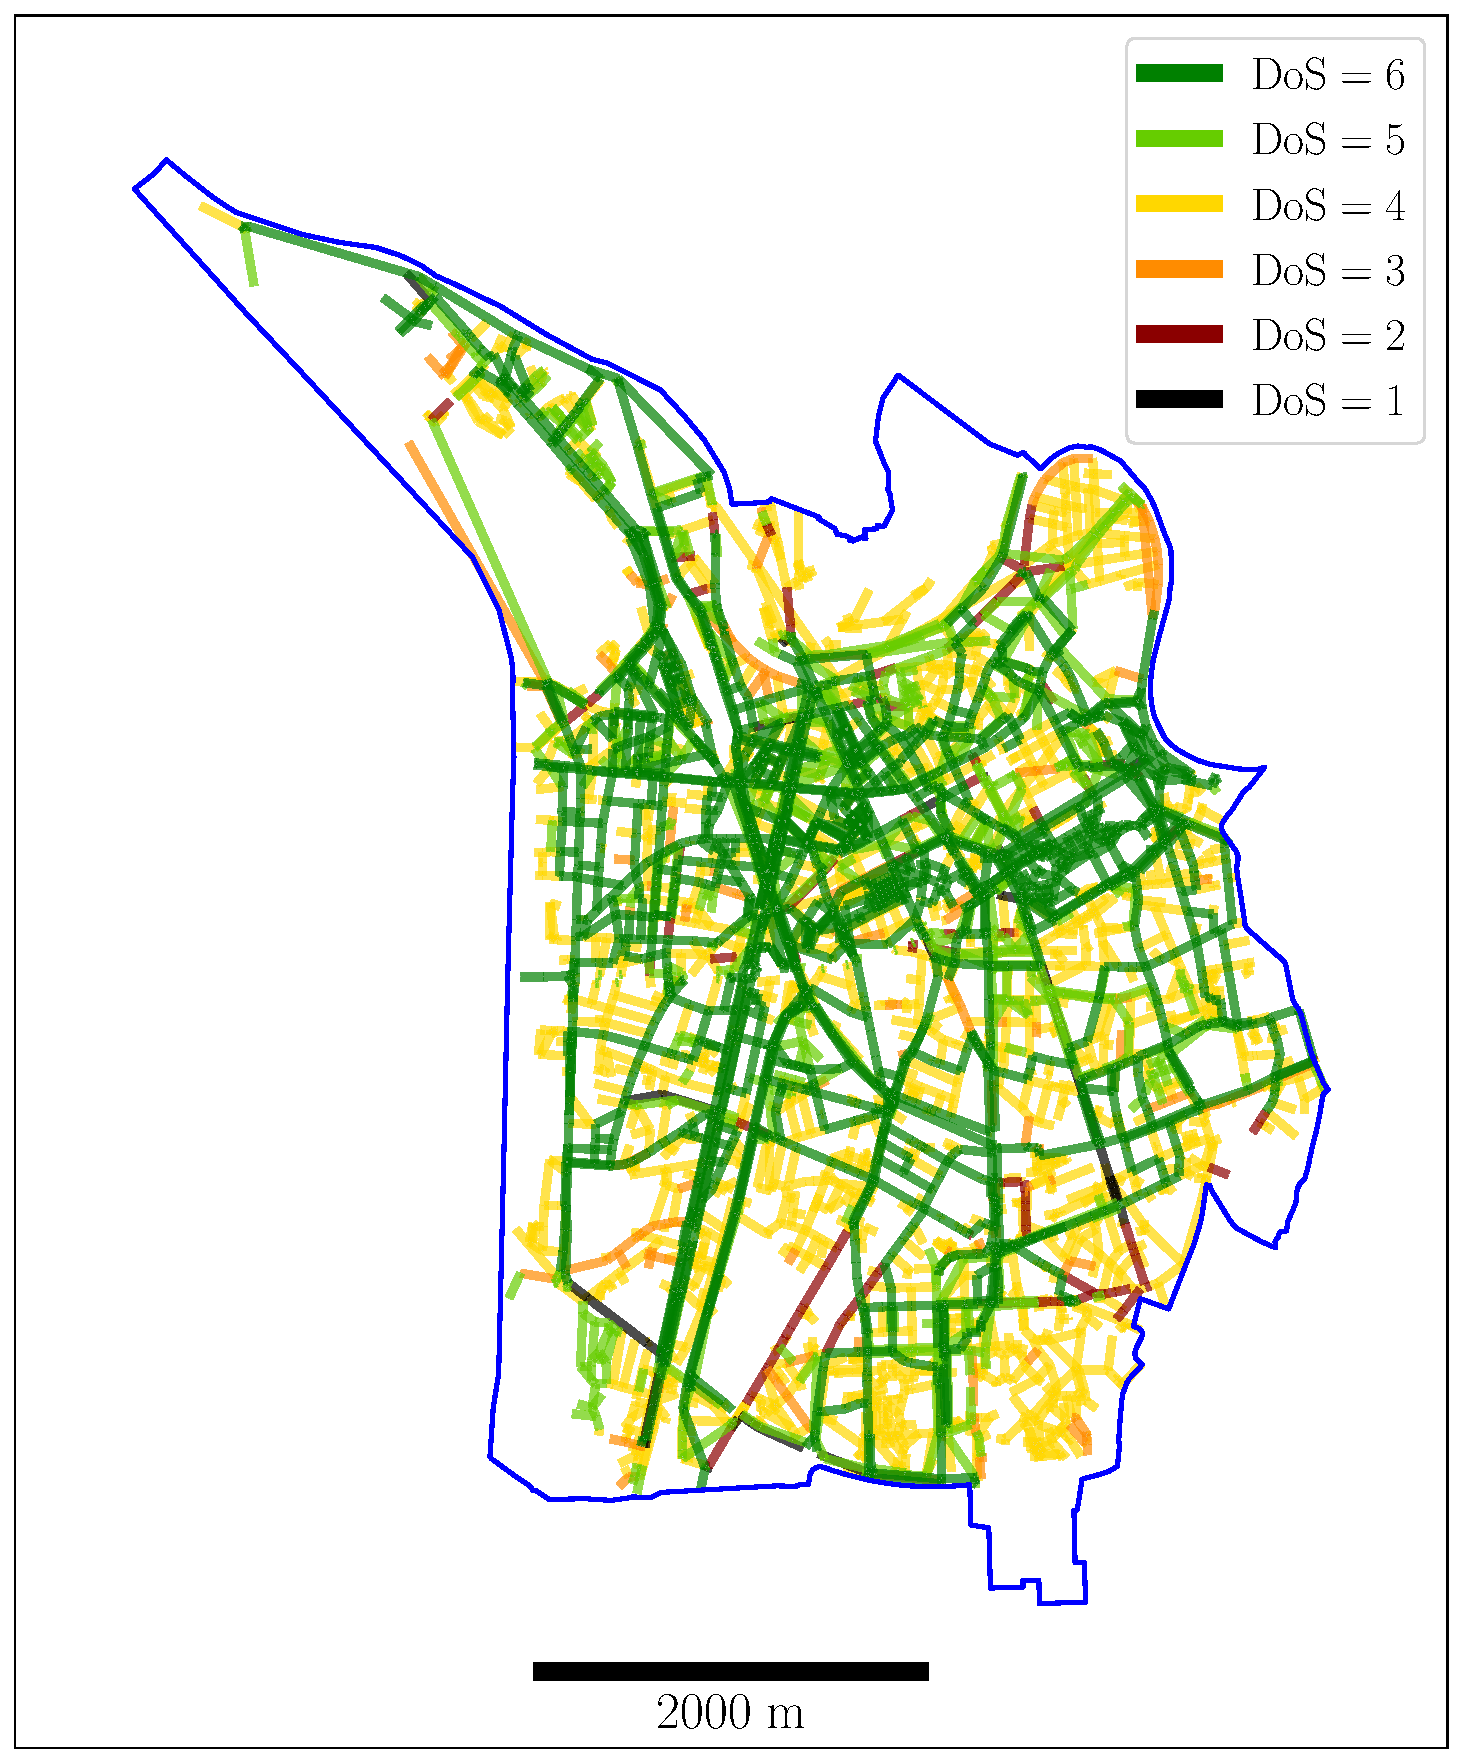
\includegraphics[width=0.29\linewidth]{Images/bike_network_mlcc_1_3.pdf}}\label{mlcc_1} \hspace{0.03\linewidth}
  % \subfloat[MLCC $\alpha=\frac{2}{5}$]{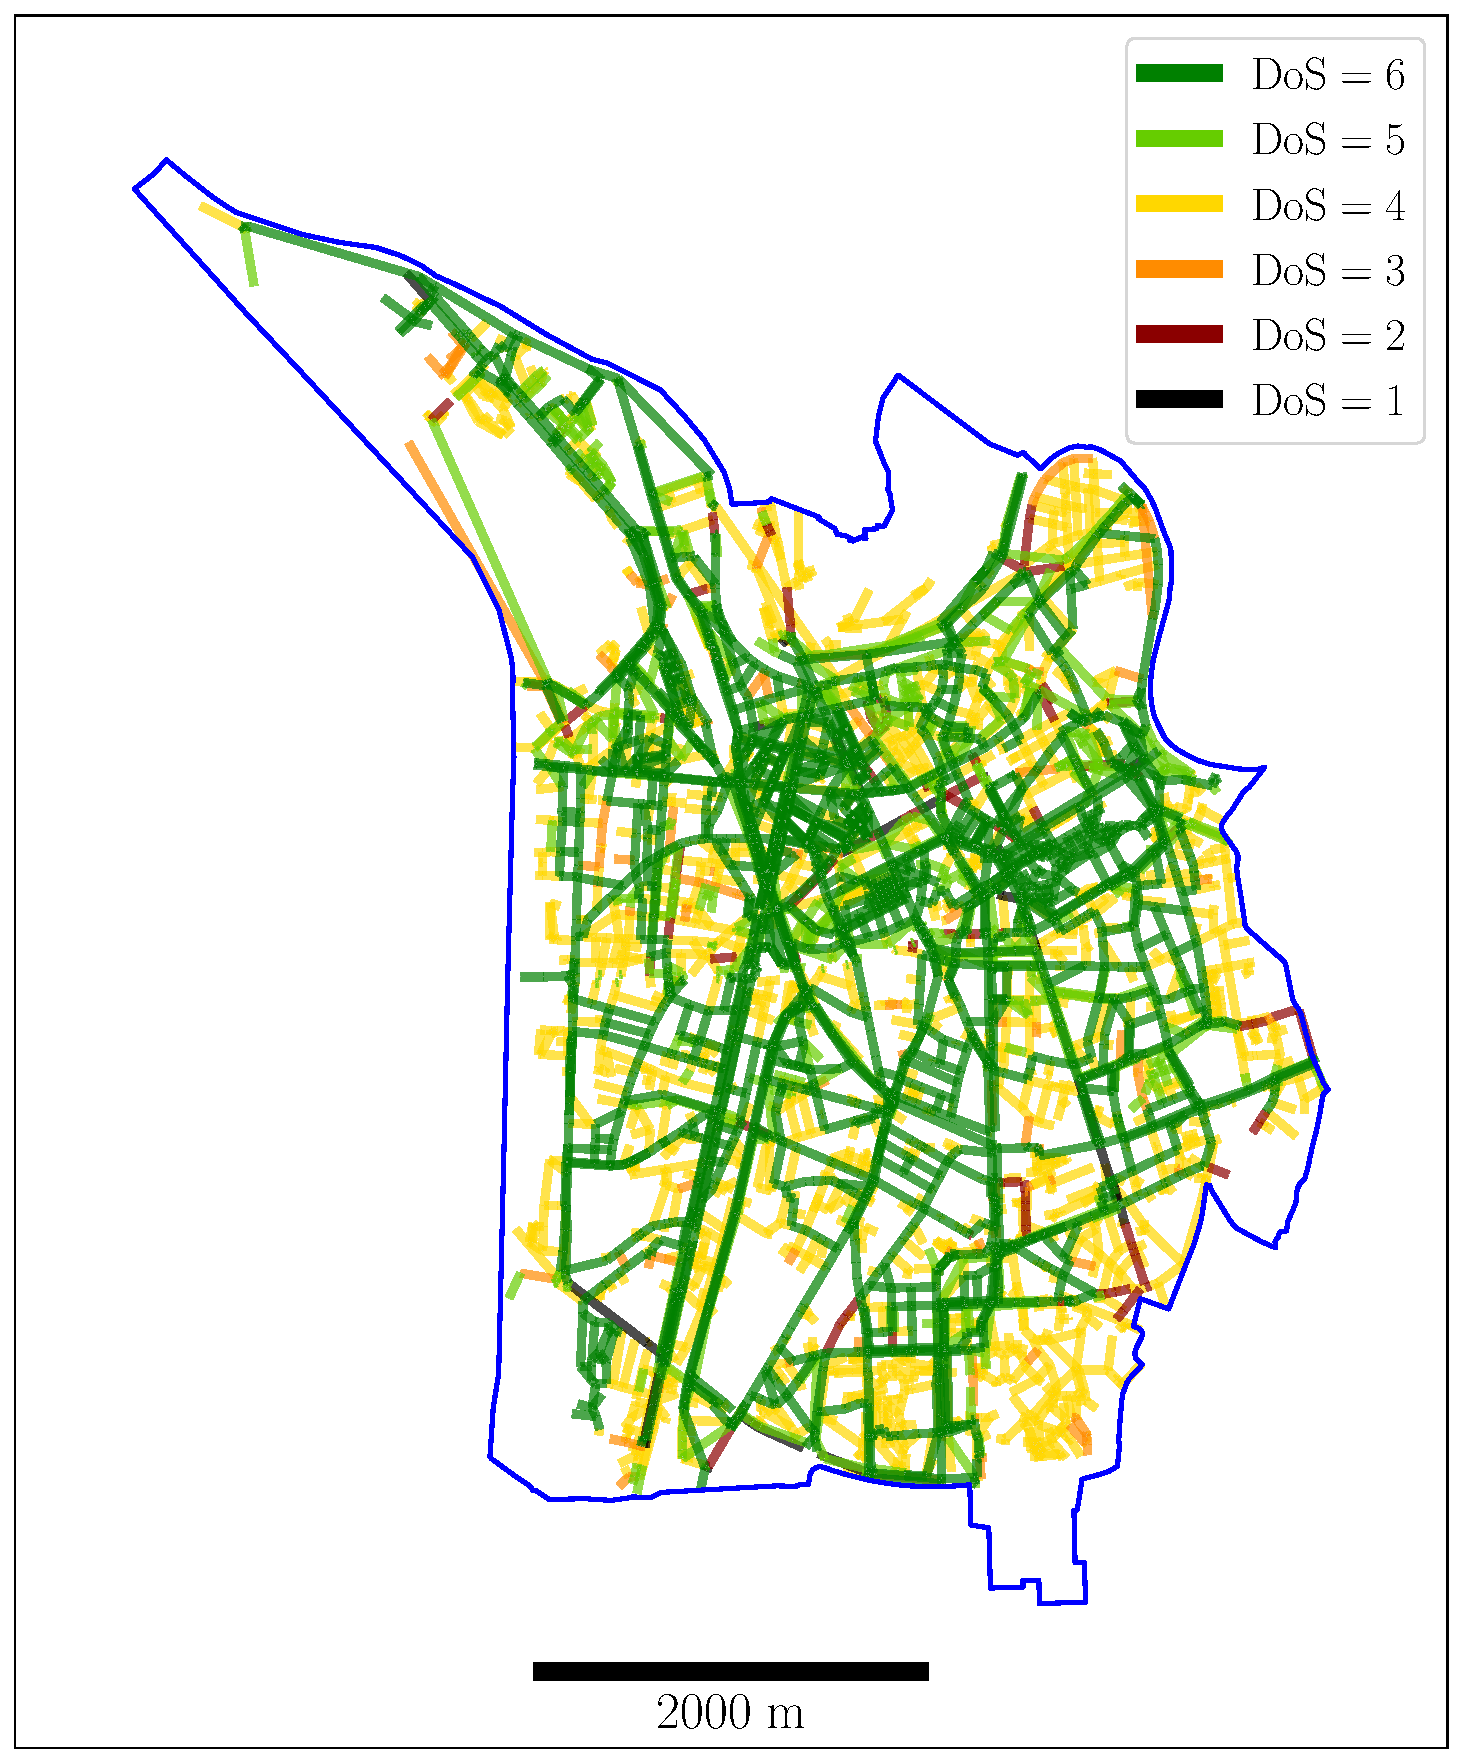
\includegraphics[width=0.29\linewidth]{Images/bike_network_mlcc_2_5.pdf}}\label{mlcc_2} \hspace{0.03\linewidth}
  % \subfloat[MLCC $\alpha=\frac{1}{2}$]{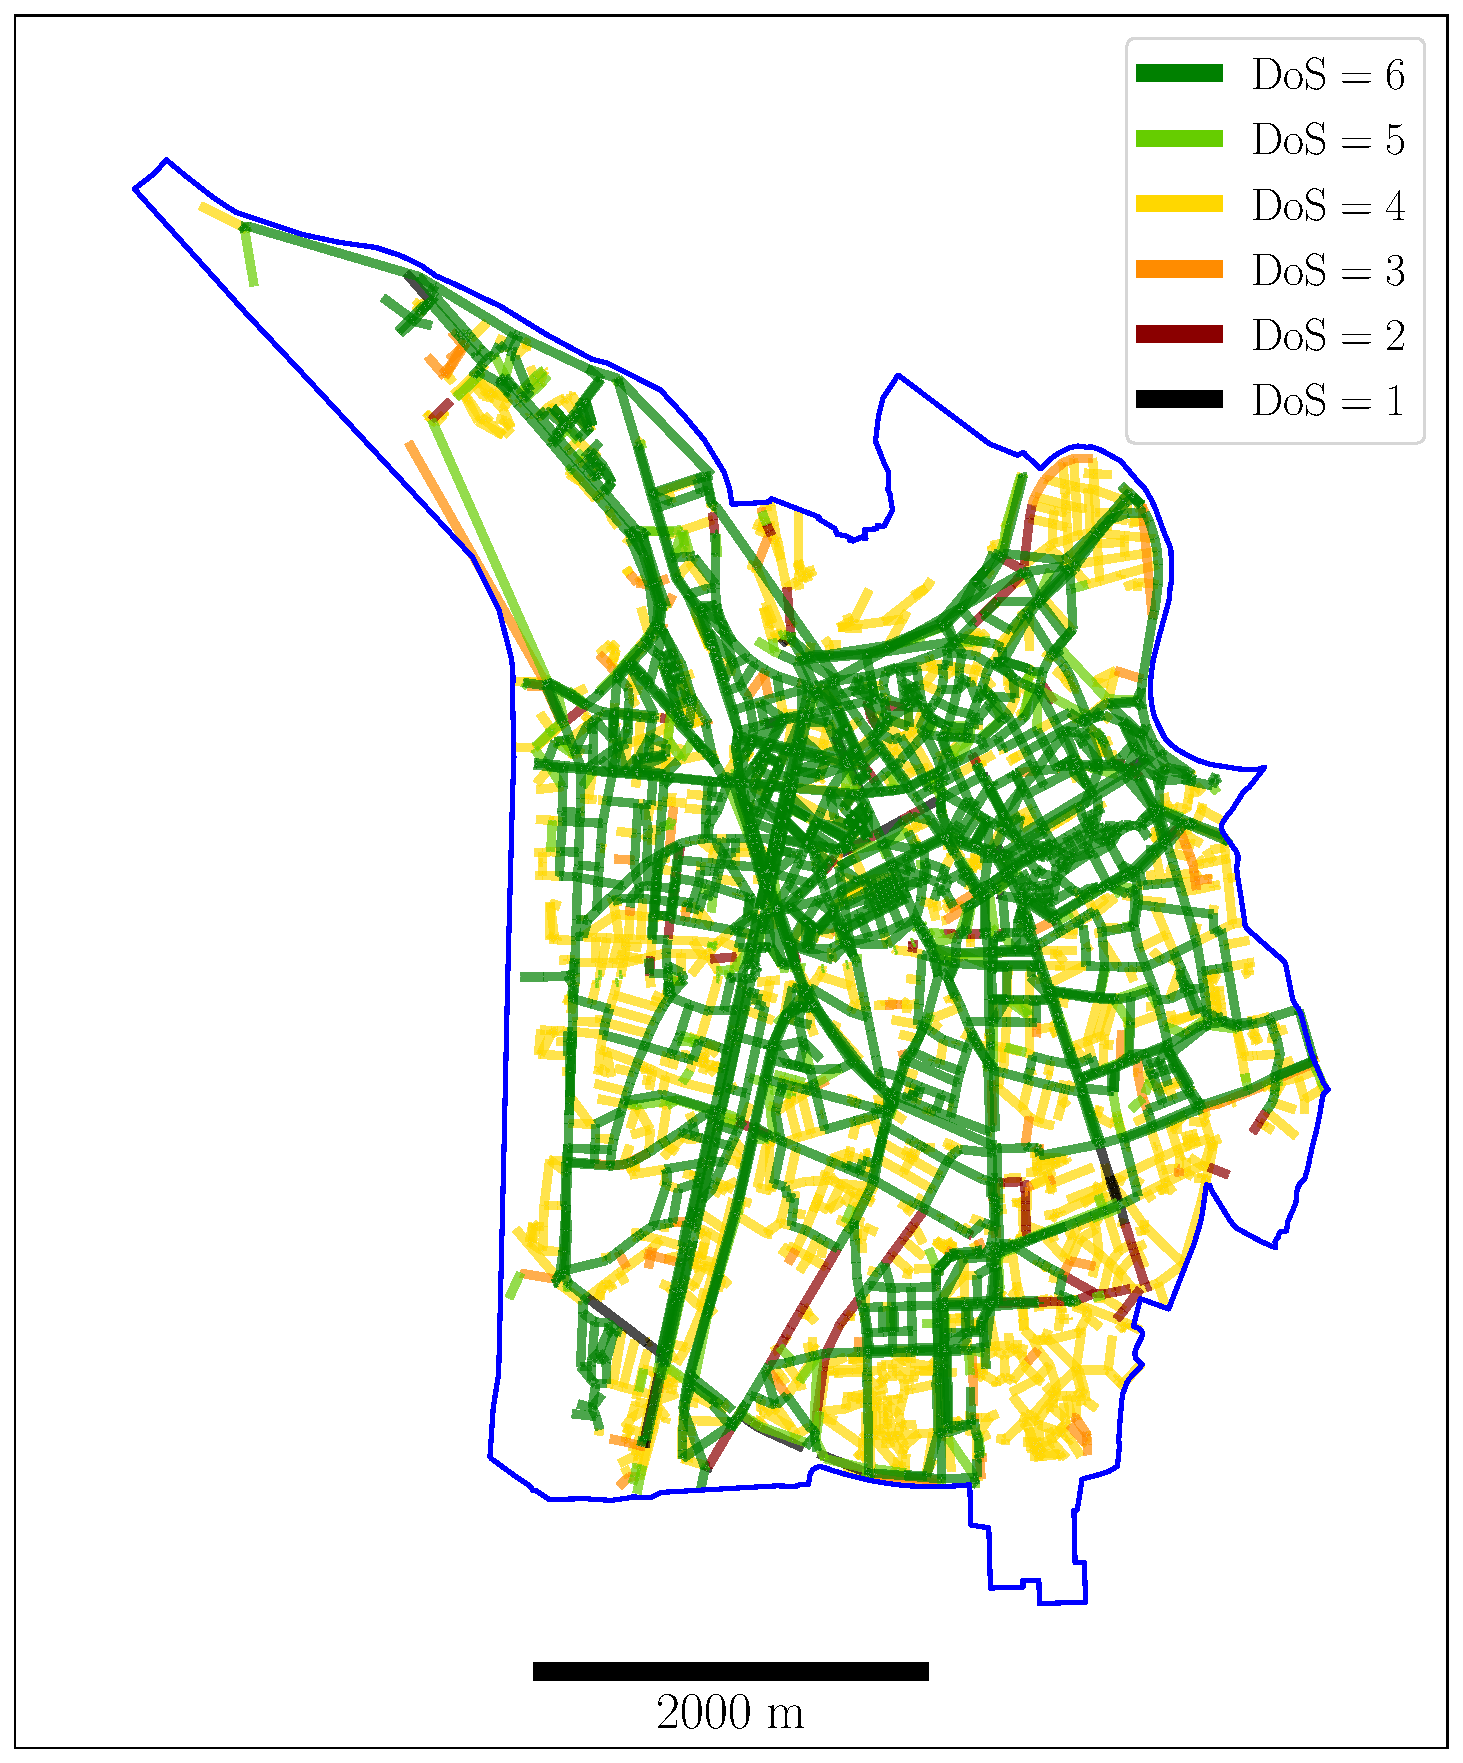
\includegraphics[width=0.29\linewidth]{Images/bike_network_mlcc_1_2.pdf}}\label{mlcc_3} \\
  \subfloat[Post-upgrade user equilibrium traffic assignment for $\epsilon^{\star}_{\frac{1}{3}}$]{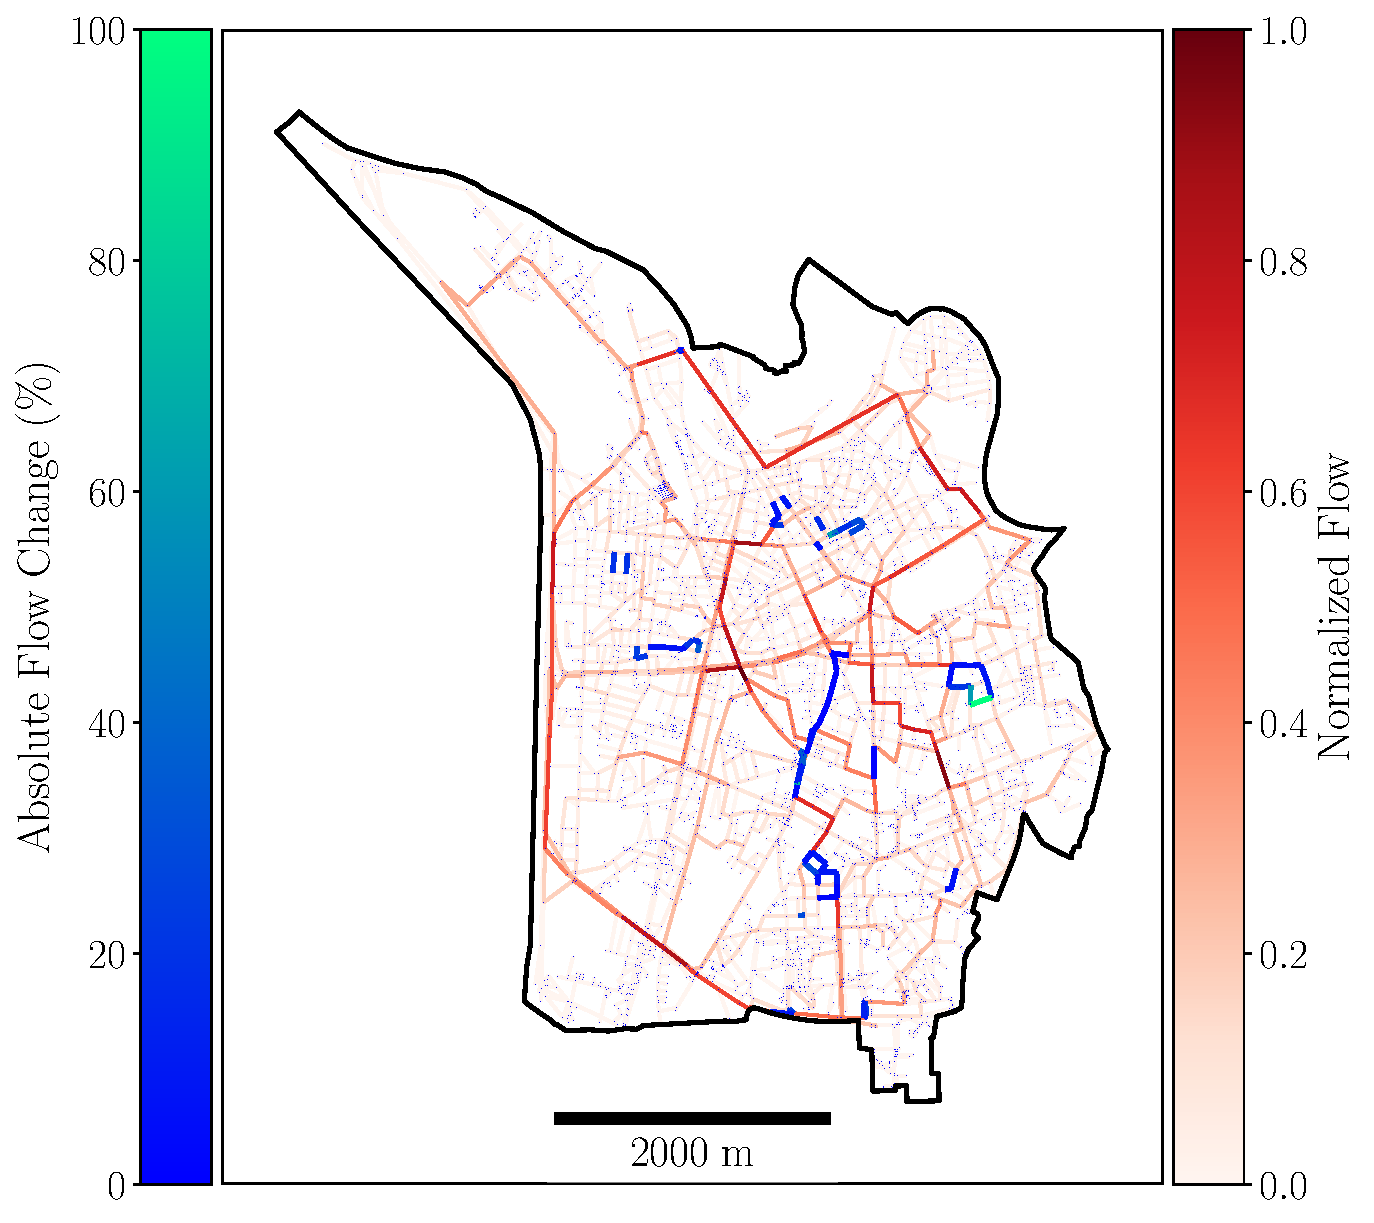
\includegraphics[width=0.32\linewidth]{Images/Grenoble_cars_flows_sga_1_3.pdf}}\label{fw_1} \hspace{0.00\linewidth}
  \subfloat[Post-upgrade user equilibrium traffic assignment for $\epsilon^{\star}_{\frac{2}{5}}$]{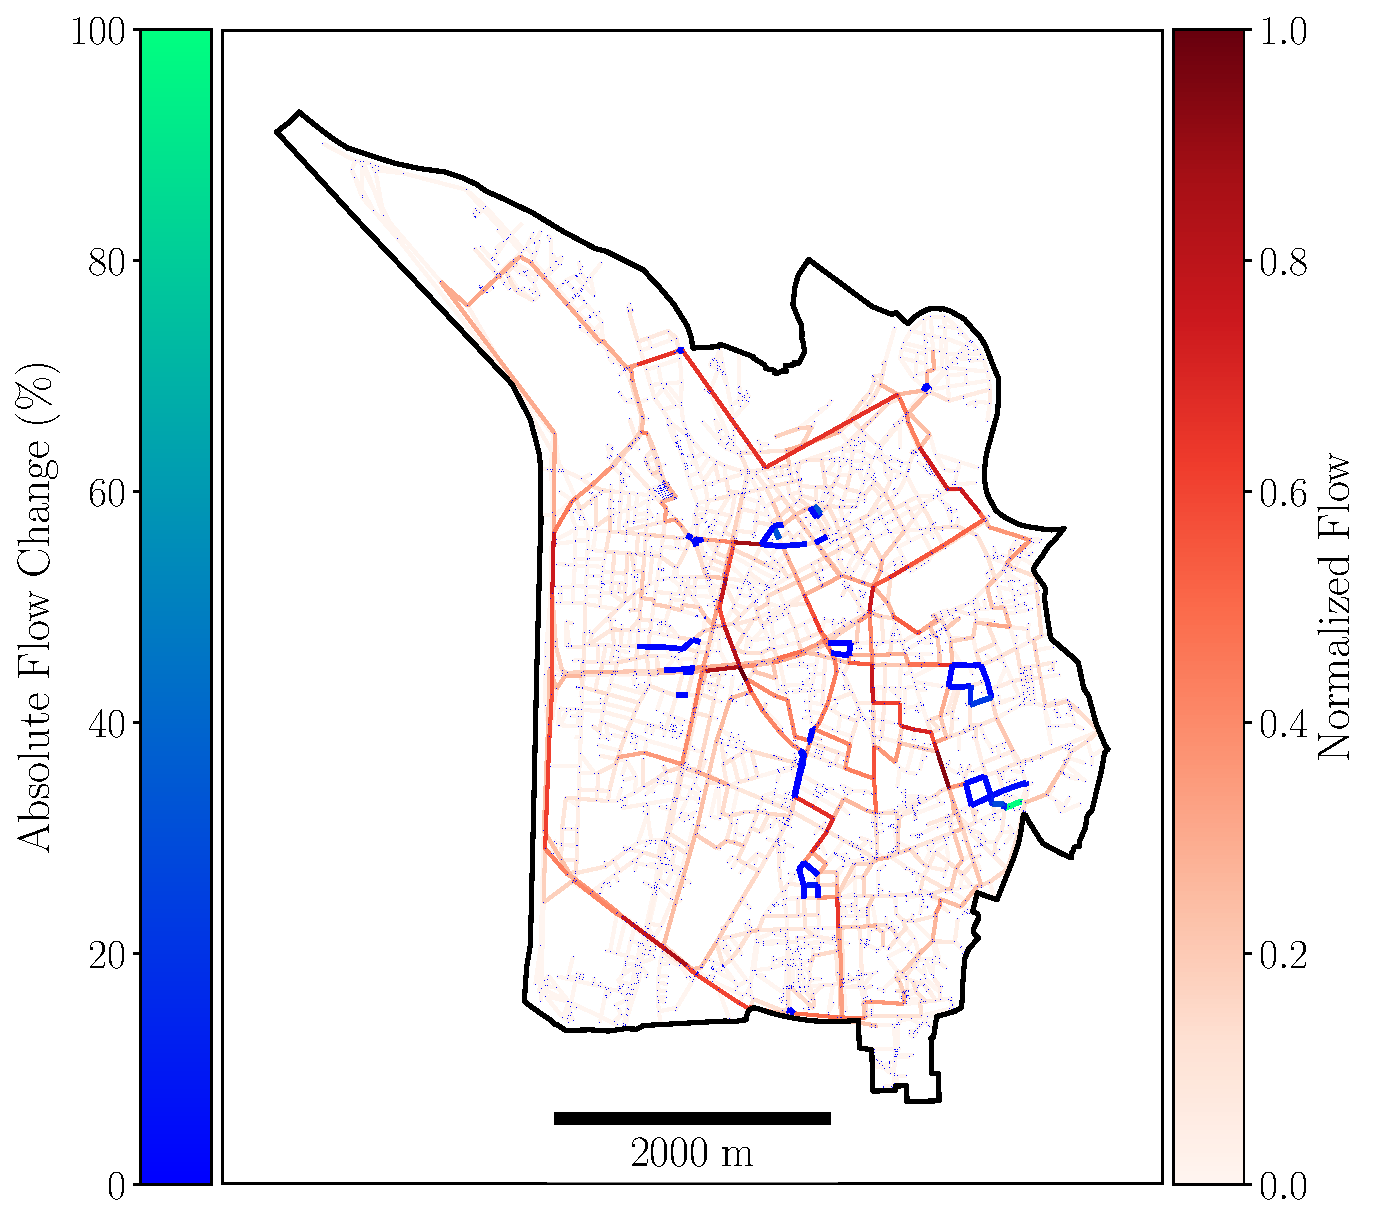
\includegraphics[width=0.32\linewidth]{Images/Grenoble_cars_flows_sga_2_5.pdf}}\label{fw_2} \hspace{0.00\linewidth}
  \subfloat[Post-upgrade user equilibrium traffic assignment for $\epsilon^{\star}_{\frac{1}{2}}$]{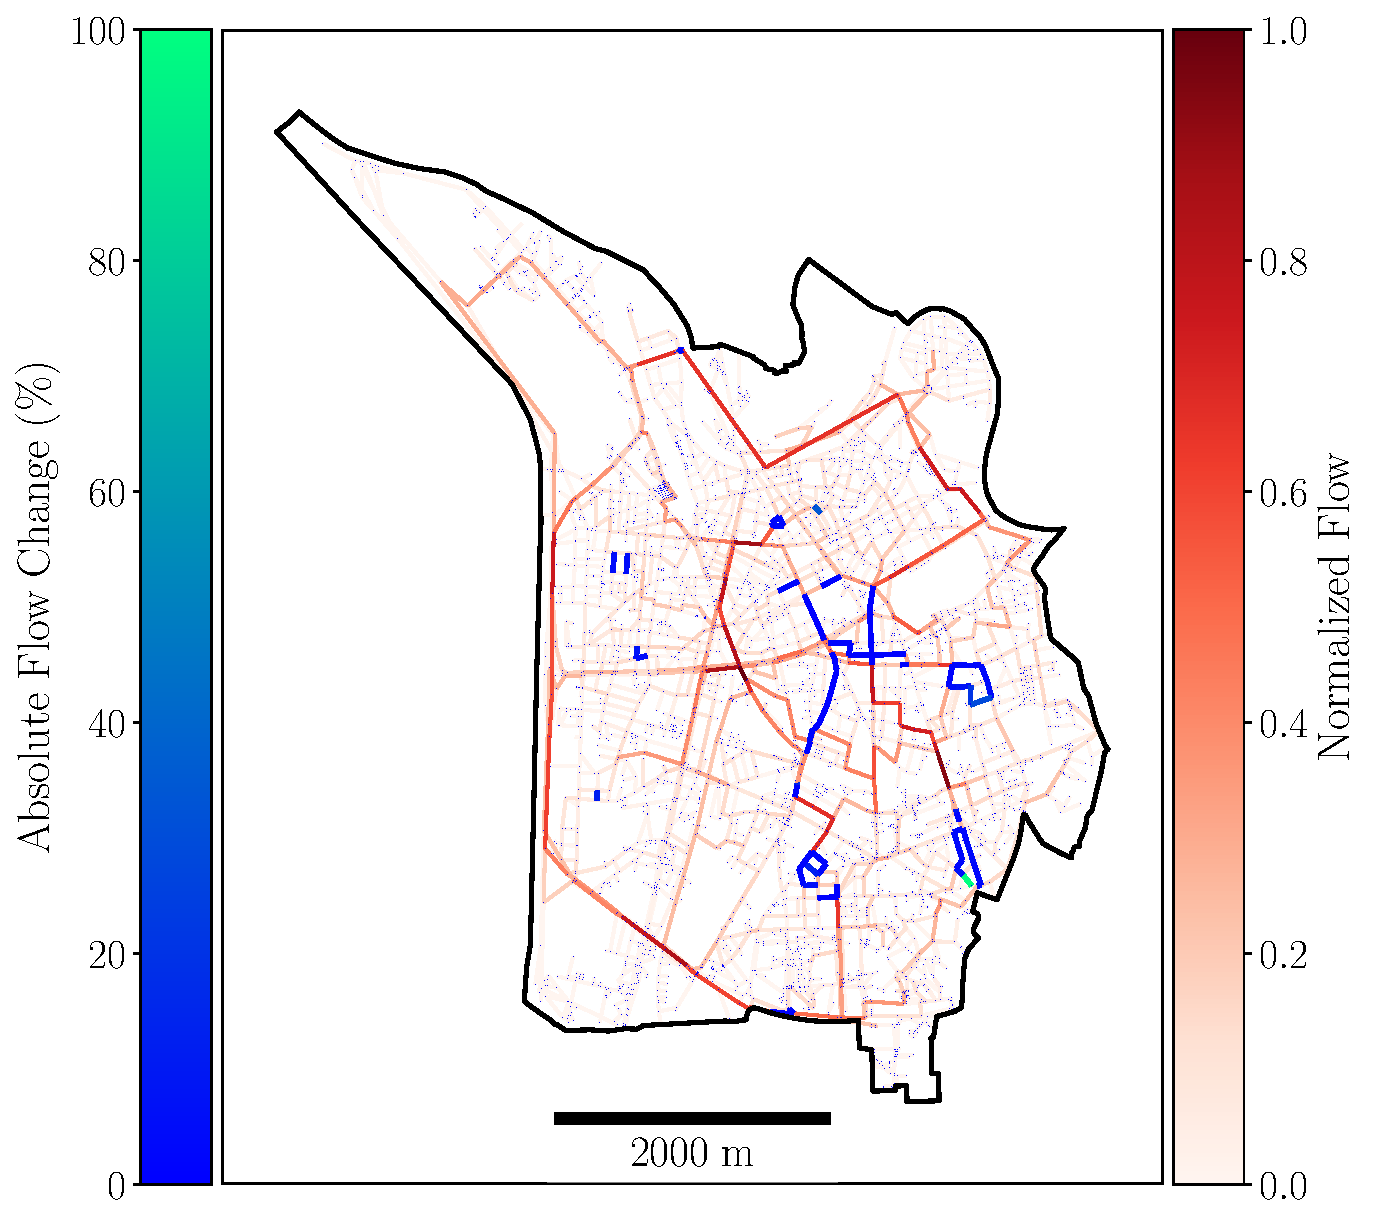
\includegraphics[width=0.32\linewidth]{Images/Grenoble_cars_flows_sga_1_2.pdf}}\label{fw_3}
  
  \caption{\footnotesize The top row shows the optimal bike lane upgrades obtained for $\epsilon^{\star}_{\alpha}$. The bottom row displays the post-upgrade UE assignment, where the left color bar highlights the percentage of the absolute flow change only for lanes with the most significant variations, while the right color bar shows the normalized flow distribution across the full network.}
  \label{bike_network_evolution}
\end{figure*}

\section{Conclusion and Future Work}
\label{conclusions}



This work presents a bi-objective optimization framework for designing safer and more efficient cycling infrastructure, demonstrated on Grenoble, France. The problem balances minimizing cyclist exposure and preserving car travel times, solved using a genetic algorithm (GA). Across varying budgets, the method identifies optimal trade-offs that significantly reduce exposure with minimal impact on car travel times, even after re-routing is accounted for through post-upgrade UE traffic assignment.

The framework offers a practical tool for planners, showing that safety and efficiency can coexist, and modest changes may promote a shift toward cycling. Future extensions could explore behavioral responses, equity, broader multi-modal systems, and alternative optimization approaches.


















%-----------------------------------------------------------------------------------------------------

\bibliographystyle{unsrt}
\bibliography{mybibfile}






\end{document}